\documentclass{elsarticle}
\usepackage{placeins}
\usepackage{amsmath}
\usepackage{amssymb}
\usepackage{graphicx}
\usepackage{subcaption}
\usepackage{lineno}
\usepackage{hyperref}
\usepackage{xcolor}
\usepackage{colortbl}
\usepackage{adjustbox}
\usepackage{multirow}
\usepackage{lscape}
\usepackage{multicol}
\usepackage{wrapfig}
\usepackage{float}
\usepackage{xparse}
\usepackage{dblfloatfix}

\setlength{\columnsep}{1cm}

\NewDocumentCommand{\evalat}{sO{\big}mm}{%
	\IfBooleanTF{#1}
	{\left. #3 \right|_{#4}}
	{#3#2|_{#4}}%
}

\DeclareMathOperator*{\argmax}{arg\,max}
\DeclareMathOperator*{\argmin}{arg\,min}

\modulolinenumbers[5]

\DeclareGraphicsExtensions{.png,.pdf}
\graphicspath{{./figures/}}

\usepackage{natbib}
\bibliographystyle{elsarticle-num}

\journal{...}
%-----------------------------------------------------
\begin{document}
%-------------------------------------------
	\begin{titlepage}
		\begin{center}
			\vspace*{1cm}
			\textbf{Robust Histogram of Oriented Gradient}
			
			\vspace{1cm}
			
		    Masoud Akhgar$^{a,b}$, Tahereh Bahraini$^{b,c}$, Hadi Sadoghi Yazdi $^{a,b,*}$\\
			\vspace{0.7cm}
			$^{a}$Department of Computer Engineering, Ferdowsi University of Mashhad, Mashhad, Iran\\
			$^{b}$Center of Excellence on Soft Computing and Intelligent Information Processing, Ferdowsi University of Mashhad, Mashhad, Iran \\
			%Tahereh Bahraini$^{a,b}$, Seyed Mohammad Hosseini$^{c}$, Mahbubeh Ghasempour$^{b,d}$, Hadi Sadoghi Yazdi$^{b,d,*}$\\
			$^{c}$Department of Electrical Engineering, Ferdowsi University of Mashhad, Mashhad, Iran\\
			%	\vspace{0.5cm}
			
		\end{center}
		Email-addresses: Masoudmdar78@gmail.com (Masoud Akhgar), bahraini.tahereh@mail\\.um.ac.ir  (Tahereh Bahraini), h-sadoghi@um.ac.ir (Hadi Sadoghi Yazdi)\\
		
		$^{*}$Corresponding author
	\end{titlepage}
%-------------------------------------------
\begin{frontmatter}
%\title{Robust Histogram of Oriented Gradient}
%--------------------------------------------------
%\author[mythirdaryaddress,mysecondaryaddress]{Masoud Akhgar}
%\ead{Masoudmdar78@gmail.com}

%\author[mymainaddress,mysecondaryaddress]{Tahereh Bahraini}
%\ead{bahraini.tahereh@mail.um.ac.ir}

%\author[mysecondaryaddress,mythirdaryaddress]{Hadi Sadoghi Yazdi\corref{mycorrespondingauthor}}
%\cortext[mycorrespondingauthor]{Corresponding author}
%\ead{h-sadoghi@um.ac.ir}

%\address[mainaddressRS]{Department of Civil Engineering, Ferdowsi University of Mashhad, Mashhad, Iran}
%\address[mysecondaryaddress]{Center of Excellence on Soft Computing and Intelligent Information Processing, Ferdowsi University of Mashhad, Mashhad, Iran}
%\address[mymainaddress]{Department of Electrical Engineering, Ferdowsi University of Mashhad, Mashhad, Iran}
%\address[mythirdaryaddress]{Department of Computer Engineering, Ferdowsi University of Mashhad, Mashhad, Iran}
%-----------------------------------------------------
%-----------------------------------------------------
\begin{abstract}
	\label{eq:area}
		Although the HOG (Histogram of Oriented Gradients) feature extraction algorithm is widely used for object detection, image classification, computer vision and image processing, it has an unfavorable result for noisy signals, due to its gradient nature.
		Therefore, the noises produced significantly influence in the outcome of HOG. In this paper, a new robust method is introduced to compute the HOG features and it is particularly studied on the noisy images to present the reduced impact of noise.
		The proposed method contains three phases leading to a higher performance against noisy images, and it is replaced in the image gradient calculation process.
		In the first step, the approximation phase is simply done by using the Maclaurin series, and it produces an acceptable outcome, promising result and execution time.
		In the following, we investigate the accuracy and correctness of the previous phase by minimizing the loss function-based optimization problem in tuning phases, in which least square and correntropy loss functions are used.
		In the last phase, we use the correntropy loss function in our method which is finally found robust against outlier noises. In this case, Gaussian and Salt and pepper noises are debated. Eventually, we compare the final result with the image histogram of gradient made by the Sobel method.
\end{abstract}
%------------------------------------------------
\begin{keyword}
Histogram of oriented gradient, Image processing, Noisy image, Correntropy loss function, Half quadratic method.
\end{keyword}
%------------------------------------------------
\end{frontmatter}
\linenumbers
%------------------------------------------------
\section{Introduction}
Histogram of oriented gradient (HOG) as an image descriptor is one of the most popular methods for feature extraction in the computer vision field, presented in 2005 by Dalal and Trigs \cite{H1}. This method first computes the gradients, then normalizes them, and finally obtains location invariant features as robust unchanged areas in the image.
Features extracted from the HOG method have various applications, such as texture classification \cite{H2}, face recognition \cite{H3}, \cite{H4}, human activity recognition \cite{H6} and vehicle detection \cite{H7}. Even with the popularity of some other methods, such as convolutional neuron network
(CNN), HOG-based methods are still desirable in these
applications due to their stable trade-off between complexity and accuracy.
Combining the HOG features in the classification structure, e.g., used Adaboost \cite{H8} and Support Vector Machines \cite{H9}, \cite{H10}, makes an object detection framework. Some researchers tried to modify and extend features using HOG descriptors \cite{H11,H12}.
%Digital images are the raw inputs for computer vision algorithms, such as HOG-based object detection systems.
HOG-based methods have limitations and disadvantages. Much research effort was devoted to optimizing HOG features' computation, increasing the processing speed, and reducing their power consumption \cite{H13,H14,H15}. 

HOG descriptor outperforms single features in most cases and most applications. But, other features combined with HOG are suggested to enhance the detection rate and provide improved performance.
In the pedestrian detection field, the cascaded features are used after the HOG frequently. The authors in \cite{H23} proposed combining HOG descriptors, shape context, shapelets, and Haar-like, named MULTIFTR features. In the continuation of this work, the MULTIFTR added to MOTION feature was presented by Walk et al. \cite{H24}, in which local-color-self-similarity, histogram of flow features \cite{H1}, and HOG were combined. 
\cite{H25} introduced new units using pairs of gradient orientations to construct histograms (CoHOG) to express complex shapes for pedestrian detection. 
A feature extraction method based on Haar-like functionality was proposed by Dollár et al. \cite{H26}. It was developed to integrate some features in different types, such as color images, gray-scale images, gradient, and directional gradient images, in a simple way named CHNFTRS. For human detection, the authors in \cite{H27} used the opponent color space (OPP) and the HOG framework and got better detection than using the RGB space alone.

Researchers conducted extensive research on HOG-based methods to overcome their limitations, as well as to make them more compatible with various applications, which has led to extensive articles in this field.
Multi-scale versions of the HOG descriptor have been previously considered. As one of the previous works, we can refer to multi-scale versions of the HOG descriptor. He et al. improved  the performance in the person detection context using a combination of the multiple scales HOG descriptors and a single encoding \cite{H16}.
Also, the authors in \cite{H17} considered two extended HOG descriptors using the multiple scales features in images and graphics applications and achieved an improved performance.
Some authors proposed the combined-based frameworks to improve the performance of HOG method, such as \cite{H18}, in which Kobayashi et el. employed HOG features in all locations of the image as the feature vectors. Then, these features were fed to Principal Component Analysis (PCA) to calculate the score vectors and reduce the number of dimensions of these features. They selected one subset of PCA-HOG features using Step-wise Forward Selection (SFS) and then applied SVM to separate pedestrian and non-pedestrian areas. Another work in pedestrian detection was done by Hua et al \cite{H19}, where a HoG-based method was proposed using a histogram of oriented spatial and temporal gradients for motion and appearance features in complex scenes.
The cascade types of rejector approach with the HOG features were introduced for face detection in \cite{H20,H21}. To speed up these methods, \cite{H22} suggested a large set of blocks for HOG features with variable locations, sizes, and aspect ratios. Then AdaBoost was applied to select the blocks in a near real-time human detection
system.

Overall, in image processing, objects can be separated in the picture using the edges, therefore it can be said that edge detection is a key aspect of image processing. Because the edges are the boundaries between objects and the background, noises generated on the images can significantly affect the object detection result using HOG. 
In our proposed method, we target some limitations of HOG and try to improve them, such as speed and accuracy, tackling with noise.
Also, the impact of the noise type and power on HOG feature extraction is studied in this paper. 
We present a robust algorithm used in calculating the gradient of signals, and the performance of the robust HOG algorithm is compared with traditional HOG descriptors in the signals and images. The proposed method can replace the operators of calculating the image gradient in the process of obtaining HOG.
Especially, it is compared with the HOG descriptor of images using Sobel gradient.

The rest of the paper is organized as follows. Section 2
discusses the backgrounds, including the image processing and HOG features. Section 3 presents the proposed robust HOG feature extraction from input images. Experimental results are presented in Section 4 and conclusions are drawn in Section 5.
%Image processing is one of the technologies in various applications of daily life such as medical images, geographical locations, astronomy and dynamic systems. Histogram of Oriented Gradients (HOG) is a significant algorithm utilized in object detection systems[1], and it detects an object using gradient of the picture. For example, it utilize in diagnosing various Stomach Cancer[2], tracking vehicles[3], diagnosing different types of skin diseases[4] and face recognition[5]. 
%----------------------------------------------------
\section{Background}

\subsection{Image and Gradient Representation}

Let $ f : \mathbb{R}^2 \rightarrow \mathbb{R} $ denote a grayscale image intensity function. Local structural information in an image can be characterized by its spatial gradient, defined as
\begin{equation}
	\nabla f(x,y) = \left( \frac{\partial f(x,y)}{\partial x}, \frac{\partial f(x,y)}{\partial y} \right).
\end{equation}

The gradient magnitude and orientation are given by
\begin{equation}
	|\nabla f(x,y)| = \sqrt{ \left( \frac{\partial f}{\partial x} \right)^2 + \left( \frac{\partial f}{\partial y} \right)^2 },
\end{equation}
\begin{equation}
	\theta(x,y) = \mathrm{atan2} \left( \frac{\partial f}{\partial y}, \frac{\partial f}{\partial x} \right).
\end{equation}

In digital images, derivatives are approximated using discrete operators. A common approach is the central difference scheme:
\begin{equation}
	\frac{\partial f}{\partial x} \approx \frac{f(x+1,y) - f(x-1,y)}{2}, \quad
	\frac{\partial f}{\partial y} \approx \frac{f(x,y+1) - f(x,y-1)}{2}.
\end{equation}

For improved robustness to noise, convolution-based operators such as Sobel filters are widely used:
\begin{equation}
	S_x =
	\begin{bmatrix}
		-1 & 0 & 1 \
		-2 & 0 & 2 \
		-1 & 0 & 1
	\end{bmatrix}, \quad
	S_y =
	\begin{bmatrix}
		-1 & -2 & -1 \
		0 & 0 & 0 \
		1 & 2 & 1
	\end{bmatrix}.
\end{equation}

\subsection{Histogram of Oriented Gradients (HOG)}

The Histogram of Oriented Gradients (HOG) is a feature descriptor that captures local shape information by encoding the distribution of gradient orientations. The image is divided into small spatial regions called \textit{cells} (typically $8 \times 8$ pixels). For each cell, a histogram over a predefined set of orientation bins is constructed.

Each pixel contributes to the histogram according to its gradient orientation, with a vote weighted by its gradient magnitude. Let $ \mathcal{C} $ denote a cell and $ B_k $ the $k$-th orientation bin. The histogram value for bin $k$ is defined as
\begin{equation}
	h_k = \sum_{(x,y) \in \mathcal{C}} |\nabla f(x,y)| \cdot \delta(\theta(x,y) \in B_k),
\end{equation}
where $ \delta(\cdot) $ is an indicator function that assigns each gradient orientation to its corresponding bin.

An illustrative example of gradient orientations, magnitudes, and their weighted contributions to orientation bins is shown in Fig.~\ref{fig1}.

To improve robustness against illumination and contrast variations, neighboring cells are grouped into larger regions called \textit{blocks}. The concatenated histogram vector within each block is normalized using $L_2$-normalization:
\begin{equation}
	\mathbf{v} \leftarrow \frac{\mathbf{v}}{\sqrt{ |\mathbf{v}|_2^2 + \epsilon^2 }},
\end{equation}
where $ \mathbf{v} $ is the block descriptor and $ \epsilon $ is a small constant for numerical stability.

The final HOG descriptor is obtained by concatenating normalized block descriptors over the entire image.

\begin{figure*}[!t]
	\centering
	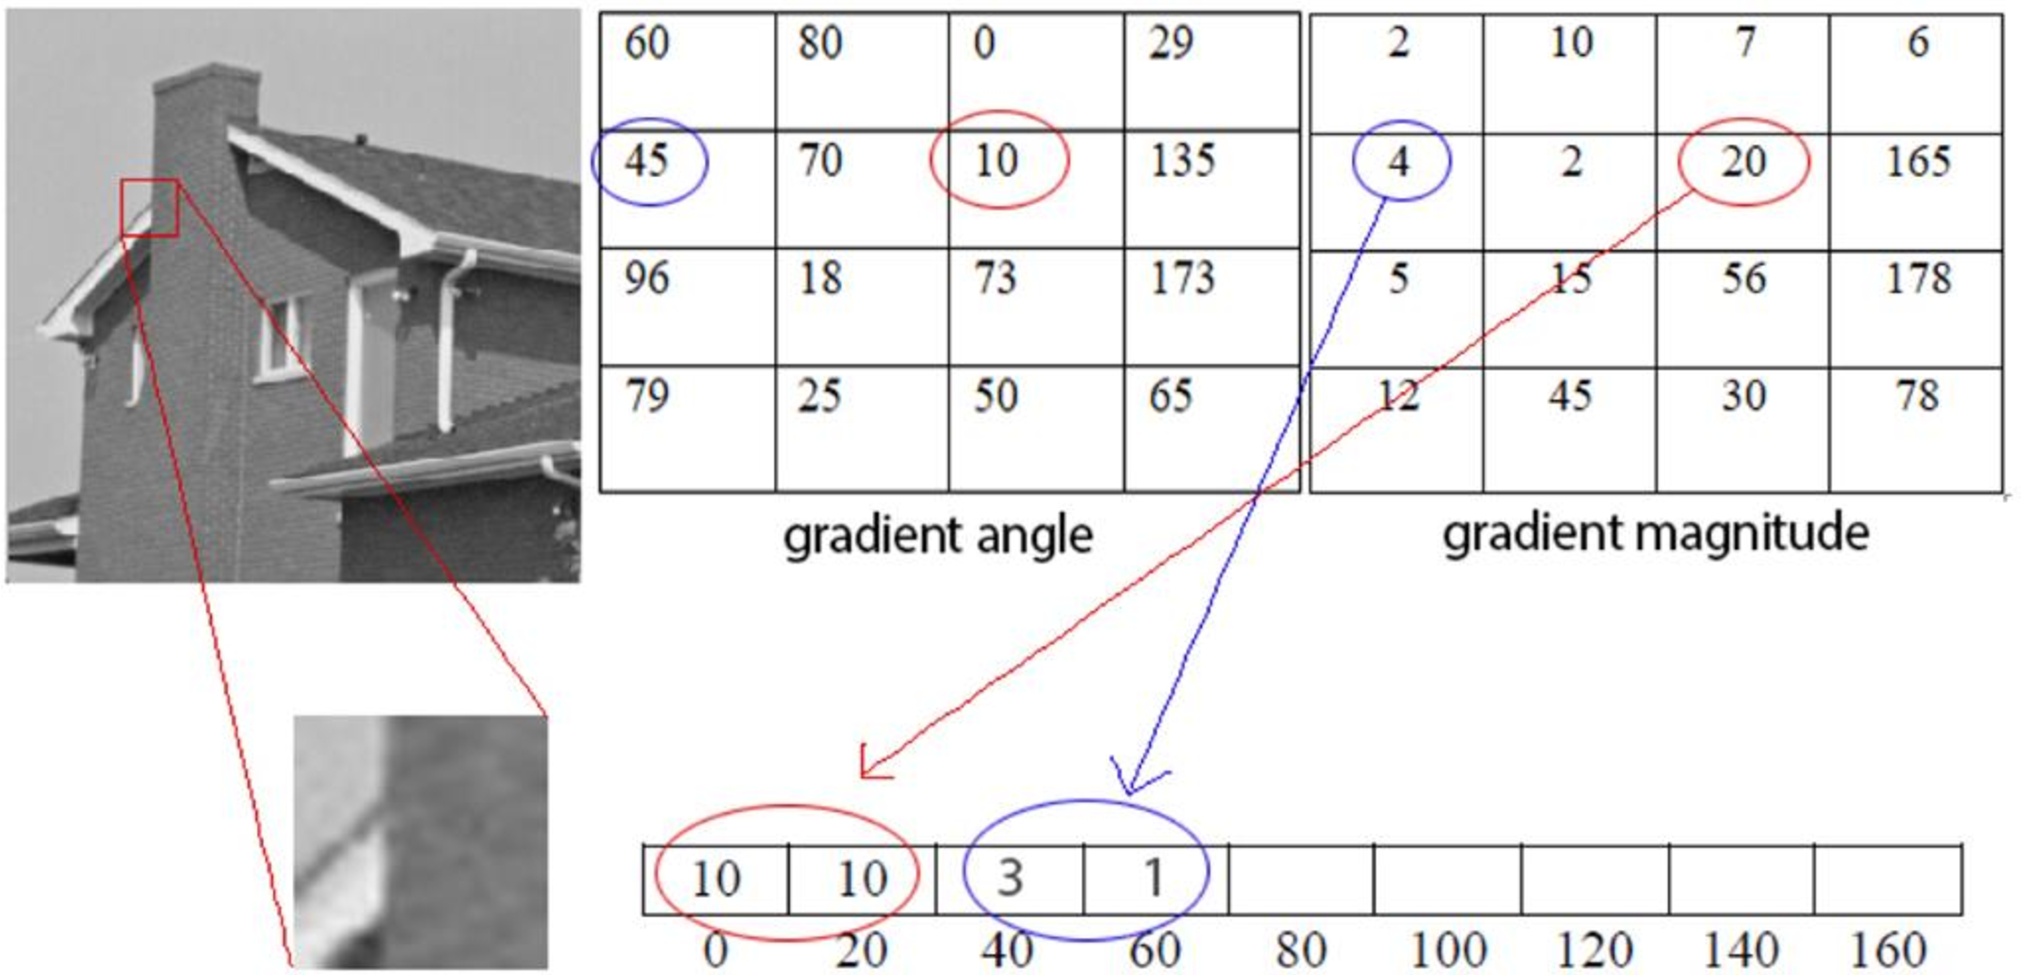
\includegraphics[width=0.75\textwidth]{Drawing1.pdf}
	\caption{Illustration of gradient orientations and magnitudes within a cell, and their weighted voting into orientation bins in the HOG descriptor.}
	\label{fig1}
\end{figure*}

%------------------------------------------------
\section{Proposed Method}

In this section, we present the proposed framework for robust gradient estimation.
While conventional methods such as finite differences and Sobel operators provide efficient approximations,
their performance degrades significantly in the presence of noise and local intensity variations.

To address this limitation, we propose a local modeling approach based on Taylor approximation,
where gradient estimation is formulated as a regression problem within a neighborhood of each pixel.
This formulation enables the incorporation of robust objective functions to reduce the influence of noise and outliers.

The overall pipeline of the proposed method is illustrated in Fig.~\ref{fig2}.
First, a local neighborhood is extracted around each pixel.
Then, a Taylor-based linear model is constructed to describe local intensity variations.
Next, a robust objective function is employed to improve estimation stability.
Finally, the resulting optimization problem is solved to obtain the gradient components.
%-----------------------------------------------------------	
\begin{figure*}[!th]
	\centering
	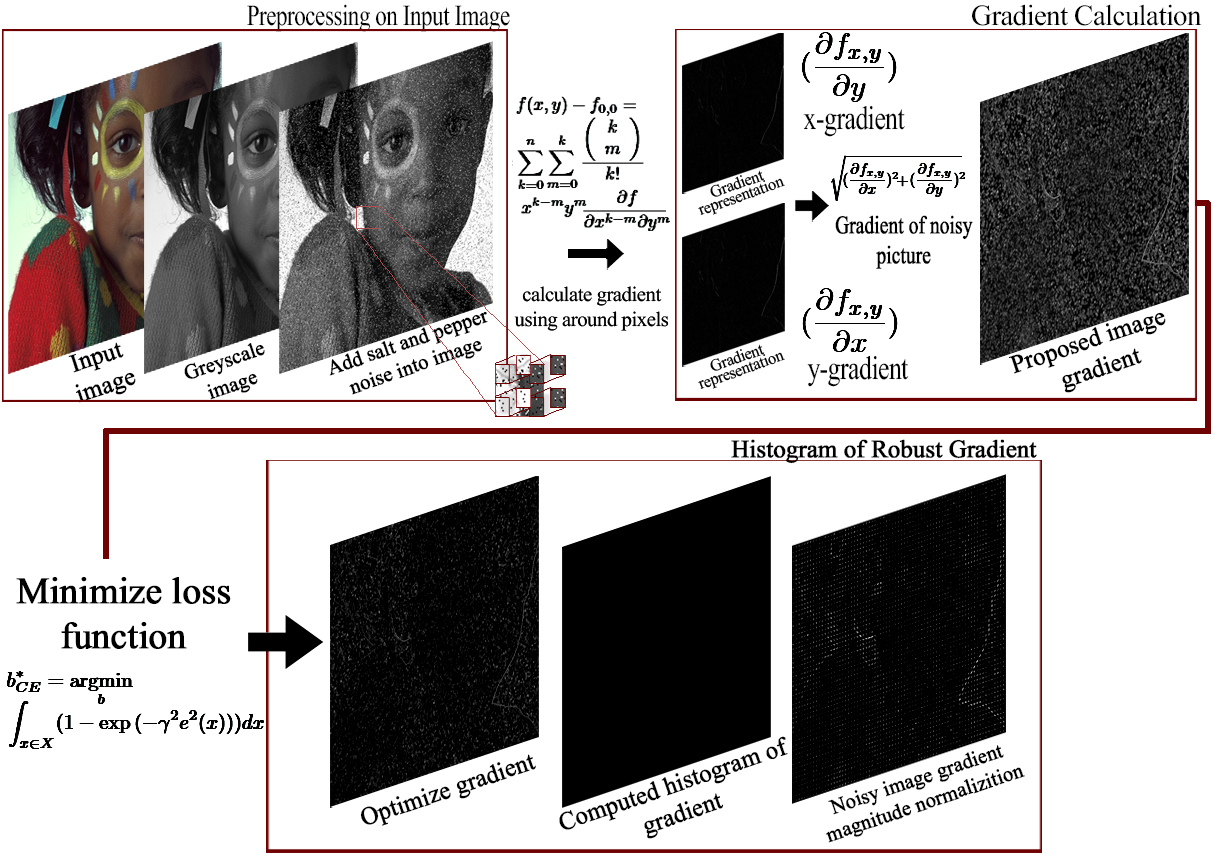
\includegraphics[height=7.5cm,width=13cm]{schematic_final.jpg}
	\caption{The block diagram of the proposed process for the calculating the robust HOG}
	\label{fig2}
\end{figure*}
%-----------------------------------------------------------

The following subsections describe each step in detail.

%----------------------------------------------------------

\subsection{Problem Formulation}
Consider a set of $n$ ordered real points such that $x_1 < x_2 < \cdots < x_n$. Let $f$ be a sufficiently smooth (i.e., continuous and differentiable up to the required order) function defined on the interval $[x_1, x_n]$. 

To approximate derivatives of $f$, we employ the Taylor expansion of $f(x)$ around a reference point $x_0 = 0$:
\begin{equation}\label{Q1}
	f(x) = f(0) + f'(0)x + \frac{f''(0)}{2!}x^2 + \cdots + \frac{f^{(z)}(0)}{z!}x^z + O(x^{z+1}),
\end{equation}
where $O(x^{z+1})$ denotes the truncation error of order $(z+1)$.

By evaluating \eqref{Q1} at symmetric points $x = \pm 1$ and truncating at order $z = 2$, we obtain:
\begin{equation}\label{Q2}
	f'(0) = \frac{f(1) - f(-1)}{2} + O(1),
\end{equation}
which corresponds to the classical central finite-difference approximation.

Since the function values are assumed to be known at discrete sample points, the derivative $f'(0)$ can be estimated numerically. In general, estimating derivatives requires constructing a system of equations obtained from Taylor expansions around zero at multiple sampling locations.

This formulation naturally recovers classical finite-difference schemes. In particular, the Sobel operator can be interpreted as a discrete first-order approximation derived from this framework by restricting the model to a minimal $3 \times 3$ neighborhood and a first-order truncation.

More generally, by evaluating the Taylor expansion at symmetric points around zero, such as $x = \pm 1, \pm 2, \ldots, \pm \frac{n}{2}$, we obtain a system of linear equations in terms of the derivatives of $f$ at the origin. Truncating the series at order $z$ and neglecting higher-order terms yields a solvable linear system for estimating derivatives.

For example, evaluating \eqref{Q1} at selected points gives:
\begin{equation}\label{Q3}
	f(1) = f(0) + f'(0) + \frac{f''(0)}{2!} + \cdots + \frac{f^{(z)}(0)}{z!} + O(1),
\end{equation}

\begin{equation}\label{Q4}
	f(-1) = f(0) - f'(0) + \frac{f''(0)}{2!} + \cdots + (-1)^z \frac{f^{(z)}(0)}{z!} + O(1),
\end{equation}

\begin{equation}\label{Q5}
	f\left(\frac{n}{2}\right) = f(0) + \frac{n}{2} f'(0) + \frac{\left(\frac{n}{2}\right)^2}{2!} f''(0) + \cdots + \frac{\left(\frac{n}{2}\right)^z}{z!} f^{(z)}(0) + O\left(\left(\frac{n}{2}\right)^{z+1}\right),
\end{equation}

\begin{equation}\label{Q6}
	f\left(-\frac{n}{2}\right) = f(0) - \frac{n}{2} f'(0) + \frac{\left(\frac{n}{2}\right)^2}{2!} f''(0) + \cdots + (-1)^z \frac{\left(\frac{n}{2}\right)^z}{z!} f^{(z)}(0) + O\left(\left(\frac{n}{2}\right)^{z+1}\right).
\end{equation}

To estimate derivatives up to order $n$, we truncate the Taylor expansion in \eqref{Q1} at $z = n$. By subtracting $f(0)$ from both sides of the resulting equations, we obtain a linear system that can be written in matrix form. Let $\mathcal{N} = \{x_1, x_2, \dots, x_M\}$ denote the set of sampling points.

\begin{equation}\label{Q9}
	\begin{aligned}
		\mathbf{A}
		\begin{bmatrix}
			f'(0) \\
			f''(0) \\
			\vdots \\
			f^{(n)}(0)
		\end{bmatrix}
		=
		\begin{bmatrix}
			f(x_1)-f(0) \\
			f(x_2)-f(0) \\
			\vdots \\
			f(x_M)-f(0)
		\end{bmatrix},
	\end{aligned}
\end{equation}
where the coefficient matrix $\mathbf{A}$ is defined as:
\[
\mathbf{A} =
\begin{bmatrix}
	x_1 & \frac{x_1^2}{2!} & \cdots & \frac{x_1^n}{n!} \\
	x_2 & \frac{x_2^2}{2!} & \cdots & \frac{x_2^n}{n!} \\
	\vdots & \vdots & \ddots & \vdots \\
	x_M & \frac{x_M^2}{2!} & \cdots & \frac{x_M^n}{n!}
\end{bmatrix}.
\]

Let the $j$-th row of $\mathbf{A}$ be:
\begin{equation}\label{Q7}
	R_j(n) = \begin{bmatrix}
		x_j & \frac{x_j^2}{2!} & \cdots & \frac{x_j^n}{n!}
	\end{bmatrix}.
\end{equation}

Define the derivative vector:
\begin{equation}
	\mathbf{d} =
	\begin{bmatrix}
		f'(0) & f''(0) & \cdots & f^{(n)}(0)
	\end{bmatrix}^T.
\end{equation}

Then each equation can be written compactly as:
\begin{equation}\label{Q8}
	f(x_j) - f(0) = R_j(n)\mathbf{d}.
\end{equation}

Solving \eqref{Q9} yields numerical estimates of derivatives at the reference point. Applying this procedure across all sample locations enables derivative computation over the entire signal.

\subsubsection{Extension to Two-Dimensional Signals}

The formulation can be extended to two-dimensional functions (e.g., images). Let $f(x,y)$ be a smooth function, and denote $f(0,0)$ by $f_{0,0}$. The Taylor expansion around $(0,0)$ is given by:
\begin{equation}\label{Q10}
	\begin{aligned}
		f(x,y) &= f_{0,0} + f_x x + f_y y \\
		&\quad + \frac{1}{2!} \left( f_{xx} x^2 + 2 f_{xy} xy + f_{yy} y^2 \right) \\
		&\quad + \frac{1}{3!} \left( f_{xxx} x^3 + 3 f_{xxy} x^2 y + 3 f_{xyy} x y^2 + f_{yyy} y^3 \right) + \cdots,
	\end{aligned}
\end{equation}
where all derivatives are evaluated at $(0,0)$.

In compact form:
\begin{equation}\label{Q11}
	f(x,y) - f_{0,0} =
	\sum_{k=1}^{\infty} \sum_{m=0}^{k}
	\frac{x^{k-m} y^{m}}{(k-m)!m!}
	\frac{\partial^{k} f}{\partial x^{k-m} \partial y^{m}}.
\end{equation}

By substituting neighboring sample points $(x_i,y_i)$ into \eqref{Q11}, we obtain a linear system:
\begin{equation}\label{Q12}
	\mathbf{B}\mathbf{d}_{2D} =
	\begin{bmatrix}
		f(x_1,y_1)-f_{0,0} \\
		\vdots \\
		f(x_n,y_n)-f_{0,0}
	\end{bmatrix},
\end{equation}
where $\mathbf{B}$ is constructed from monomials of $(x_i,y_i)$ and $\mathbf{d}_{2D}$ contains partial derivatives.

Increasing the number of terms improves accuracy but also increases computational complexity and sensitivity to noise. Near boundaries, where symmetric neighborhoods are unavailable, one-sided approximations must be used. This trade-off is analogous to polynomial fitting: higher-order models provide better approximation but are more sensitive to noise. This formulation also enables the integration of robust estimation techniques, which will be discussed in the next subsection.

We consider both the squared loss and a correntropy-induced loss to solve the resulting linear system. The squared loss provides an efficient baseline but is sensitive to outliers. To enhance robustness, we adopt a correntropy-based formulation, which can be interpreted as an adaptive reweighting of the squared loss. Both formulations are retained for comparison. We first present the squared loss and then its correntropy-based extension.

\subsection{Least Squares-Based HOG}

To enhance robustness against noise and truncation errors in the Taylor-based formulation presented in the previous subsection, we reformulate the approximation model by explicitly introducing a residual (bias) term. Specifically, we consider:
\begin{equation}\label{QSM}
	f(x) = \hat{f}(x) + b
\end{equation}
where $\hat{f}(x)$ is a truncated Taylor expansion of $f(x)$ around the reference point $x_0 = 0$, and $b$ represents the residual approximation error, which implicitly captures the neglected higher-order terms, i.e., $b \approx O(x^{z+1})$. Using the Taylor expansion up to order $z$, we have:
\begin{equation}
	\hat{f}(x)=\sum_{n=0}^{z}\frac{f^{(n)}(0)}{n!}x^n
\end{equation}

To estimate the optimal value of $b$, we formulate the following least-squares optimization problem:
\begin{equation}\label{Q14_1}
	b^*_{LS}=\argmin_{b}\int_{x\in X} l(e(x)),dx
\end{equation}
where the residual error is defined as:
\begin{equation}
	e(x)=f(x)-\hat{f}(x)-b
\end{equation}
and $X$ denotes the domain of interest.

By adopting the least-squares loss function $l(e(x)) = e^2(x)$, we obtain:
\begin{equation}\label{Q15_1}
	b^*_{LS}=\argmin_{b}\int_{x\in X}\left(f(x)-\hat{f}(x)-b\right)^2 dx
\end{equation}

We truncate the Taylor expansion up to the fourth order and explicitly parameterize higher-order contributions as:
\begin{equation}\label{Q16_1}
	\hat{f}(x)\approx f(0)+f'(0)x+\frac{f''(0)}{2!}x^2+\alpha_1 x^3+\alpha_2 x^4
\end{equation}
where $\alpha_1$ and $\alpha_2$ model higher-order effects beyond the second derivative.

Substituting \eqref{Q16_1} into the objective function yields:
\begin{equation}\label{Q17_1}
	b^*_{LS}=\argmin_{b}\int_{x\in X}\Big(f(x)-\big[f(0)+f'(0)x+\frac{f''(0)}{2!}x^2+\alpha_1 x^3+\alpha_2 x^4 + b \big]\Big)^2 dx
\end{equation}

By taking the derivative with respect to $b$ and setting it to zero, we obtain:
\begin{equation}\label{Q18_1}
	\int_{x\in X}\Big(f(x)-\hat{f}(x)-b\Big) dx = 0
\end{equation}
which leads to the closed-form solution:
\begin{equation}\label{Q19_1}
	b = \frac{1}{|X|}\int_{x\in X} \big(f(x)-\hat{f}(x)\big),dx
\end{equation}

To estimate the unknown parameters, we define the following sub-problems:

\begin{enumerate}
	
	\item \textbf{$b_{LS}$ sub-problem:}
	\begin{equation}\label{Q20_1}
		b_{LS} \approx f(x)-f(0)-f'(0)x-\frac{f''(0)}{2!}x^2
	\end{equation}
	
	\item \textbf{$f'(0)$ sub-problem:}
	
	In practice, instead of solving the full linear system in \eqref{Q9}, we adopt a computationally efficient approximation:
	\begin{equation}\label{Q22_1}
		f'(0)\approx \frac{f(h)-f(-h)}{2h}
	\end{equation}
	
	\item \textbf{$f''(0)$ sub-problem:}
	\begin{equation}\label{Q23_1}
		f''(0)\approx \frac{f(h)-2f(0)+f(-h)}{h^2}
	\end{equation}
	
	\item \textbf{$\alpha$ sub-problem:}
	
	The higher-order coefficients are estimated via a least-squares formulation:
	\begin{equation}\label{Q21_1}
		\alpha = (A^{T}A)^{-1}A^{T}b
	\end{equation}
	where $\alpha=\begin{bmatrix}\alpha_1 \ \alpha_2\end{bmatrix}$ and the design matrix is defined as:
	\[
	A = \begin{bmatrix} x^3 & x^4 \end{bmatrix}.
	\]
	
\end{enumerate}

The two proposed methods are summarized in Tables~\ref{tab:alg1} and~\ref{tab:alg2}. 
The first method provides a non-iterative solution, while the second method iteratively updates the parameters until convergence.

%------------------------------------------
\begin{table}[t]
	\centering
	\normalsize
	\caption{Algorithm I: Non-iterative least squares-based HOG}
	\label{my-labelI}
 \begin{adjustbox}{width=0.7\linewidth}
		\begin{tabular}{l}
			\hline
			\textbf{Input:} $f(x)$, $h$, $D_x=\{x_i\}_{i=1}^{M}$ \\
			\textbf{Output:} $f'(x)$ and $f''(x)$ \\
			\hline
			\textbf{1:} Estimate $f'(x)$ using \eqref{Q22_1} \\
			\textbf{2:} Estimate $f''(x)$ using \eqref{Q23_1} \\
			\hline
		\end{tabular}
	\end{adjustbox}
\end{table}


%------------------------------------------
\begin{table}[t]
	\centering
	\normalsize
	\caption{Algorithm II: Iterative least squares-based HOG}
	\label{my-labelII}
	\begin{adjustbox}{width=0.9\linewidth}
		\begin{tabular}{l}
			\hline
			\textbf{Input:} $f(x)$, $h$, $D_x=\{x_i\}_{i=1}^{M}$ \\
			\textbf{Output:} $f'(x)$ and $f''(x)$ \\
			\textbf{Initialization:} Initialize $b$, $\alpha$, $f'(x)$, $f''(x)$ \\
			\hline
			\textbf{Repeat until convergence:} \\
			\textbf{1:} Update $b$ using \eqref{Q20_1} \\
			\textbf{2:} Update $f'(x)$ using \eqref{Q22_1} \\
			\textbf{3:} Update $f''(x)$ using \eqref{Q23_1} \\
			\textbf{4:} Update $\alpha$ using \eqref{Q21_1} \\
			\hline
		\end{tabular}
	\end{adjustbox}
\end{table}
%------------------------------------------

%------------------------------------------------
\subsection{Correntropy-Based Robust Formulation}

The conventional squared loss is highly sensitive to outliers, since large deviations can dominate the optimization process. To enhance robustness, we adopt a correntropy-based loss function, which effectively suppresses the influence of large errors.

The correntropy-induced loss is defined as
\begin{equation}
	l(e(x)) = 1 - \exp\big(-\gamma^2 e^2(x)\big),
\end{equation}
where $e(x)$ denotes the approximation error.

Accordingly, the parameter estimation problem is formulated as
\begin{equation}\label{Q24_1_new}
	b^*_{CE} =
	\argmin_{b}
	\int_{x \in X}
	\left(1 - \exp\big(-\gamma^2 e^2(x)\big)\right)\, dx.
\end{equation}

Since the constant term does not affect the solution, \eqref{Q24_1_new} is equivalent to
\begin{equation}\label{Q25_1_new}
	b^*_{CE} =
	\argmax_{b}
	\int_{x \in X}
	\exp\big(-\gamma^2 e^2(x)\big)\, dx.
\end{equation}

To solve \eqref{Q25_1_new}, we employ the half-quadratic (HQ) optimization framework using the conjugate representation
\begin{equation}\label{Q26_1_new}
	\exp\big(-\gamma^2 e^2(x)\big) =
	\sup_{p(x) < 0}
	\left\{
	\gamma^2 e^2(x)\, p(x) - \Phi\big(p(x)\big)
	\right\},
\end{equation}
where
\begin{equation}
	\Phi(p) = -p \log(-p) + p.
\end{equation}

Substituting \eqref{Q26_1_new} into \eqref{Q25_1_new} leads to the joint optimization problem
\begin{equation}\label{Q28_1_new}
	\{b^*_{CE}, p^*(x)\} =
	\argmax_{b,\, p(x)}
	\int_{x \in X}
	\left(
	\gamma^2 e^2(x)p(x) - \Phi(p(x))
	\right)\, dx.
\end{equation}

This problem can be efficiently solved via alternating optimization. Specifically, fixing $p(x)$ reduces the problem to a weighted least-squares form:
\begin{equation}\label{Q29_1_new}
	b^*_{CE} =
	\argmin_{b}
	\int_{x \in X}
	\big(-p(x)\big)\, e^2(x) \, dx,
\end{equation}
where $-p(x) > 0$ acts as an adaptive weight.

Using a second-order Taylor expansion around $a$, the approximation error can be expressed as
\begin{equation}\label{Q30_1_new}
	e(x) \approx
	f(x) - f(a)
	- f'(a)(x-a)
	- \frac{f''(a)}{2}(x-a)^2.
\end{equation}

By substituting \eqref{Q30_1_new} into \eqref{Q29_1_new}, we obtain a weighted least-squares problem, from which the parameter vector $\boldsymbol{\beta}$ is estimated as
\begin{equation}\label{Q30_2_new}
	\boldsymbol{\beta} =
	(B^T W B)^{-1} B^T W \mathbf{b},
\end{equation}
where $W = \mathrm{diag}(-p(x_i))$ is the diagonal weight matrix.

The first- and second-order derivatives are then computed as
\begin{equation}\label{Q30_3_new}
	f'(0) =
	\frac{1}{2}
	\Big[
	f(1) - f(-1)
	+ \mathbf{z}(-1)\boldsymbol{\beta}
	-
	\mathbf{z}(1)\boldsymbol{\beta}
	\Big],
\end{equation}

\begin{equation}\label{Q30_4_new}
	f''(0) =
	2\Big[
	f(1) - f(0)
	+ \mathbf{z}(1)\boldsymbol{\beta}
	- f'(0)
	\Big],
\end{equation}
where
\begin{equation}
	\mathbf{z}(x) =
	\begin{bmatrix}
		x^3 & x^4
	\end{bmatrix},
	\quad
	\boldsymbol{\beta} =
	\begin{bmatrix}
		\beta_1 \\
		\beta_2
	\end{bmatrix}.
\end{equation}

Next, fixing $b_{CE}$, the auxiliary variable is updated by solving
\begin{equation}\label{Q31_1_new}
	p^*(x) =
	\argmax_{p(x)}
	\left(
	\gamma^2 e^2(x)p(x) - \Phi(p(x))
	\right),
\end{equation}
which yields the closed-form solution
\begin{equation}\label{Q32_1_new}
	p^*(x) = -\exp\big(-\gamma^2 e^2(x)\big).
\end{equation}

Therefore, $p(x)$ acts as an adaptive weight that automatically down-weights large errors, improving robustness against outliers.

The overall iterative procedure is summarized in Table~\ref{tab:robust_hog}.

\begin{table}[t]
	\centering
	\normalsize
	\caption{Proposed Iterative Robust HOG based on Correntropy}
	\label{tab:robust_hog}
	\begin{tabular}{l}
		\hline
		\textbf{Input:} $f(x)$, $D_x = \{x_i\}_{i=1}^M$, $\gamma^2$ \\ 
		\textbf{Output:} $f'(x)$, $f''(x)$ \\
		
		\textbf{Initialize:} $\boldsymbol{\beta}$, $p(x)$ \\
		
		1: Compute $B$ \\
		2: \textbf{repeat} \\
		3: \quad Compute $W = \mathrm{diag}(-p(x_i))$ \\
		4: \quad Update $\boldsymbol{\beta}$ using \eqref{Q30_2_new} \\
		5: \quad Compute $e(x)$ using \eqref{Q30_1_new} \\
		6: \quad Update $p(x)$ using \eqref{Q32_1_new} \\
		7: \textbf{until convergence} \\
		\hline
	\end{tabular}
\end{table}

Repeated iterations may introduce numerical round-off errors due to matrix inversion. Therefore, the number of iterations should be properly controlled to ensure stable convergence and accurate estimation.


\subsection{Huber Loss Formulation}

While the squared loss provides optimal performance under Gaussian noise and the correntropy-based loss offers strong robustness to outliers, an intermediate alternative can be obtained using the Huber loss. This loss function combines the advantages of both quadratic and linear penalties, leading to a balanced trade-off between sensitivity and robustness.

Given the residual $e_i$, the Huber loss is defined as
\begin{equation}
	\rho_{\delta}(e_i) =
	\begin{cases}
		\frac{1}{2} e_i^2, & |e_i| \leq \delta, \\
		\delta \left( |e_i| - \frac{1}{2} \delta \right), & |e_i| > \delta,
	\end{cases}
\end{equation}
where $\delta$ is a positive threshold parameter controlling the transition between the quadratic and linear regimes.

Using this loss, the estimation problem can be formulated as
\begin{equation}
	\min_{\mathbf{x}} \sum_{i=1}^{N} \rho_{\delta}(e_i),
\end{equation}
where $e_i$ denotes the $i$-th residual derived from the linearized model.

The Huber loss behaves quadratically for small residuals, preserving efficiency under near-Gaussian noise, while transitioning to a linear penalty for large deviations, thereby reducing the influence of outliers. From an optimization perspective, this formulation can be interpreted as a compromise between least-squares estimation and more robust approaches such as correntropy-based methods.
This formulation allows us to bridge the gap between purely quadratic and highly robust loss functions, providing additional flexibility in handling moderately corrupted observations.
%------------------------------------------
\section{Experimental Results}

In this section, a comprehensive experimental evaluation is conducted to assess the effectiveness of the proposed methods for HOG feature extraction under both noise-free and noisy conditions. The experiments are designed to validate the proposed framework from different perspectives, including the accuracy of derivative estimation, the influence of algorithmic parameters, robustness against image degradation, and comparison with conventional edge detection approaches.

The experimental evaluation consists of several stages. First, synthetic functions with known analytical derivatives are employed to validate the correctness and convergence behavior of the proposed derivative estimation framework. Then, the effect of the main parameters and computational complexity of the proposed methods are investigated. Finally, the proposed approaches are evaluated on real-world images under different noise conditions and compared with the Sobel operator as a representative conventional method.

All experiments are performed under identical computational conditions for all compared methods to ensure a fair evaluation. The detailed description of datasets, noise generation procedures, and implementation settings is provided in the following subsection.

To evaluate robustness against image degradation, two common noise types, namely Gaussian and salt-and-pepper noise, are added to the original images at different intensity levels, generating multiple degraded versions of each image. Gaussian noise is generated by sampling from a zero-mean normal distribution with different variance levels, whereas salt-and-pepper noise is introduced by randomly replacing a proportion of pixels with the minimum or maximum intensity values. The noise levels are selected to evaluate the performance of the proposed methods under different degradation scenarios.

All methods, including the proposed approaches and the Sobel operator as a baseline, are implemented in Python and executed under identical computational conditions to ensure a fair comparison. The experiments analyze the effectiveness of the proposed methods under various noise conditions and investigate the influence of key parameters, particularly the neighborhood size parameter $h$, on the quality of HOG extraction.

For visual comparison, the original images and their noisy counterparts are presented in Fig.~\ref{fig:dataset_noise}, enabling a direct qualitative assessment of the effect of noise and the robustness of the evaluated methods.

\FloatBarrier
\begin{figure*}[!t]
	\centering
	
	\begin{subfigure}{\textwidth}
		\centering
		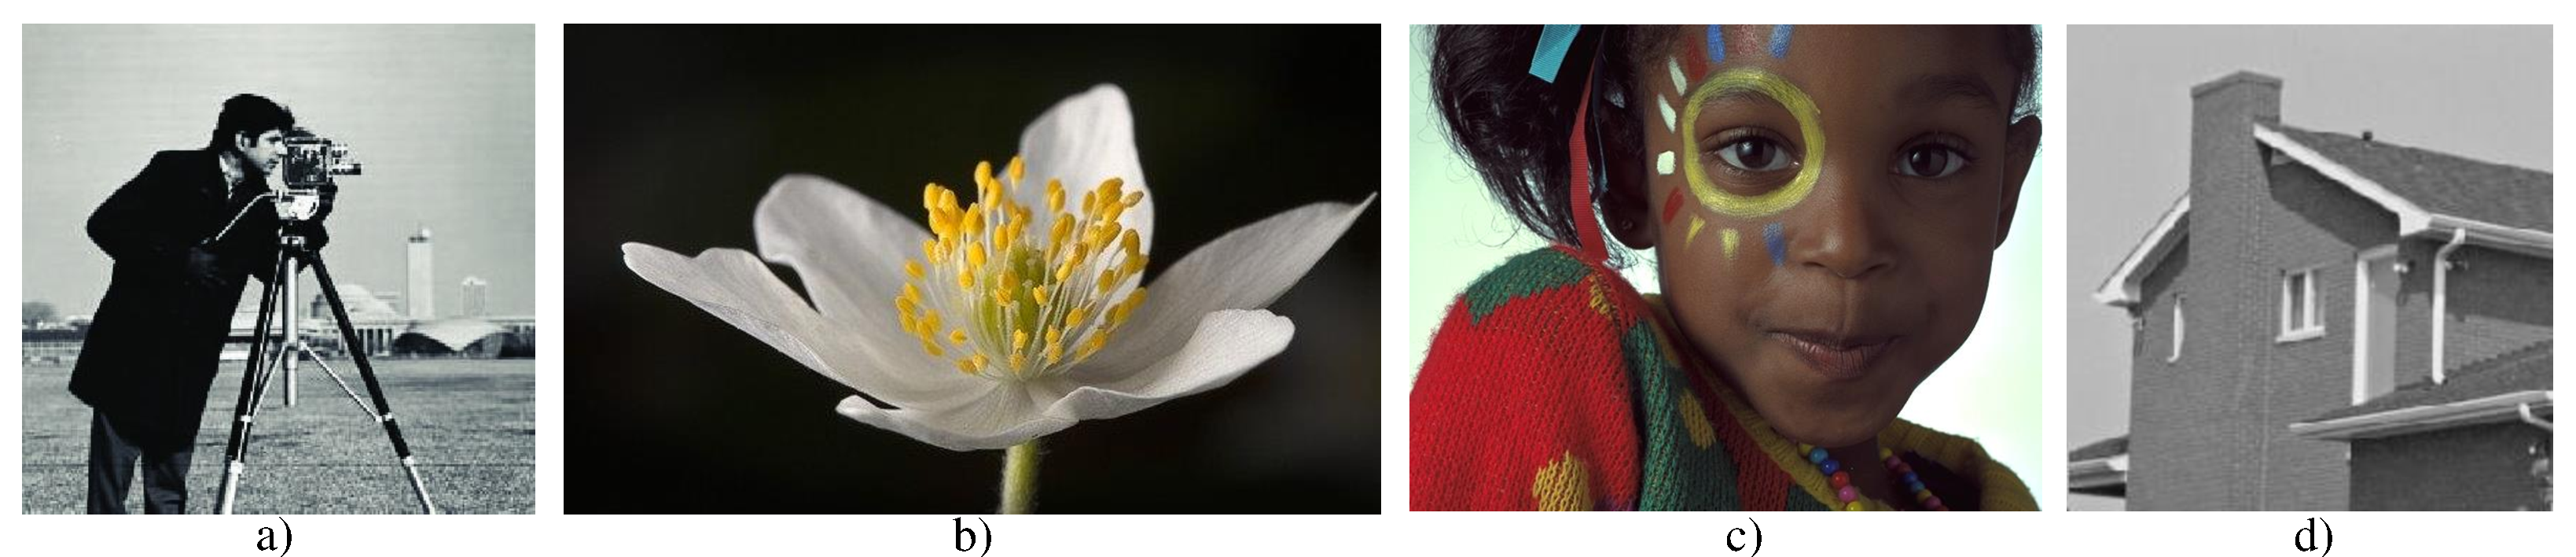
\includegraphics[width=\textwidth]{initial_images1.pdf}
		\caption{Original images}
	\end{subfigure}
	
	\vspace{2mm}
	
	\begin{subfigure}{\textwidth}
		\centering
		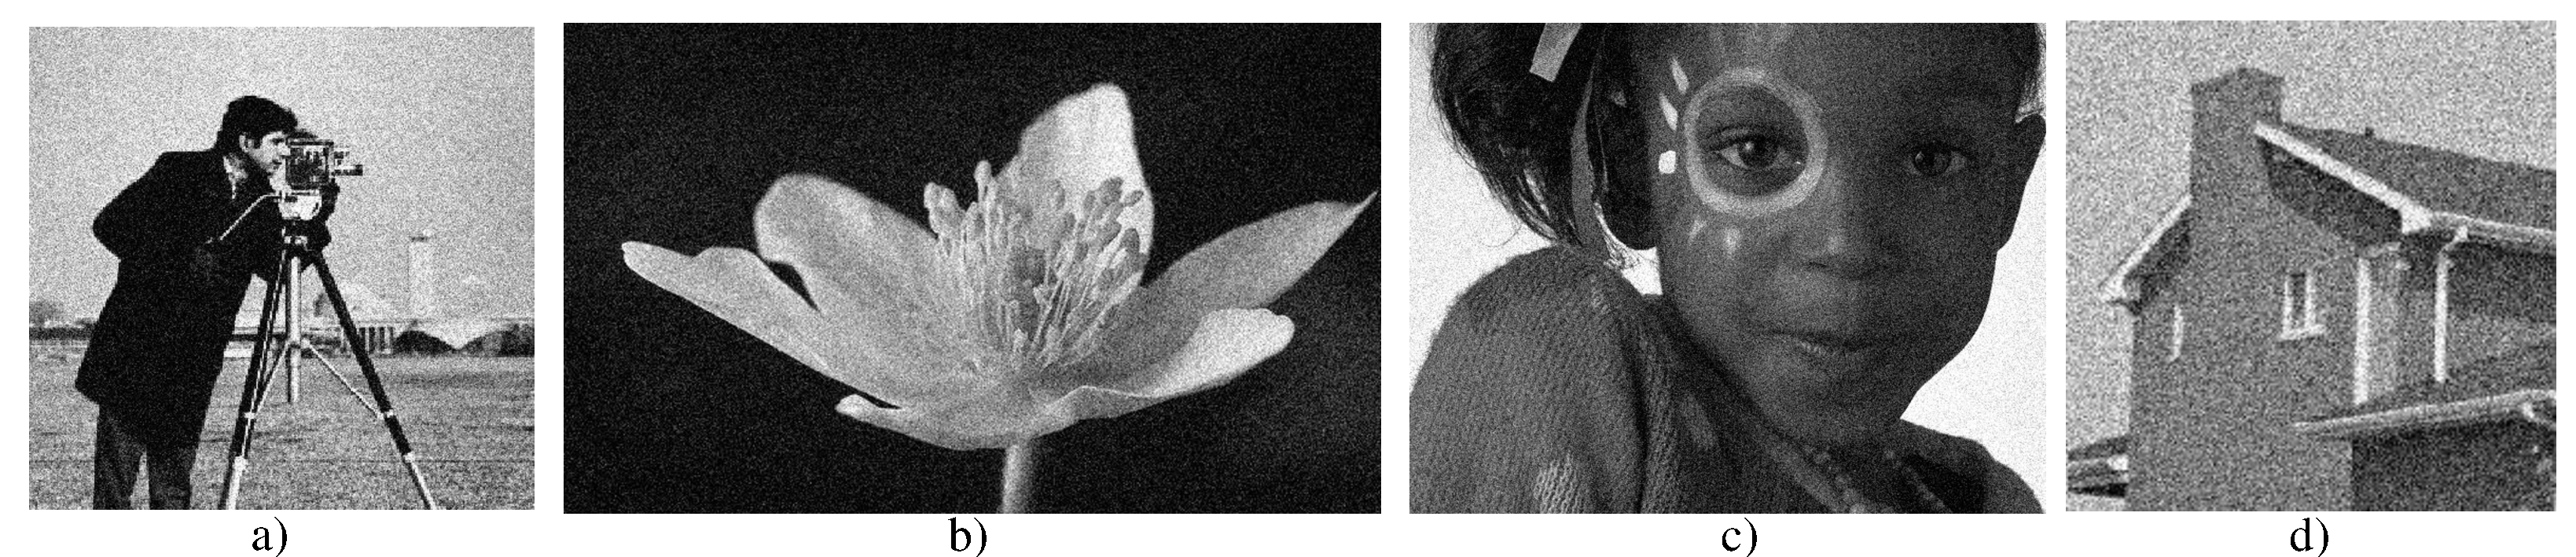
\includegraphics[width=\textwidth]{initial_images2.pdf}
		\caption{Images corrupted with Gaussian noise}
	\end{subfigure}
	
	\vspace{2mm}
	
	\begin{subfigure}{\textwidth}
		\centering
		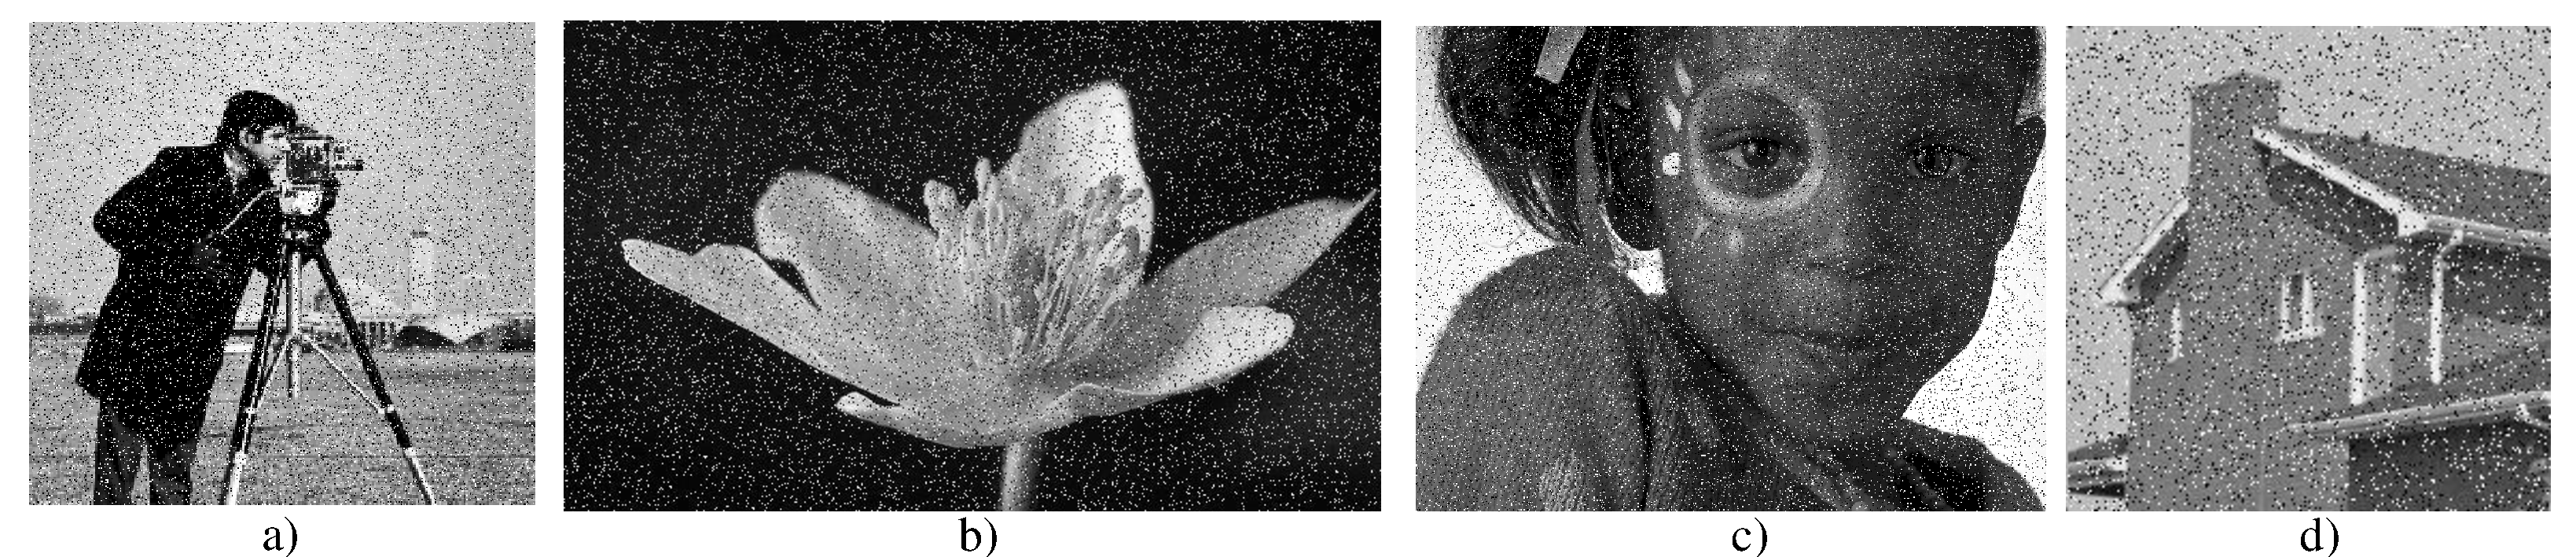
\includegraphics[width=\textwidth]{initial_images3.pdf}
		\caption{Images corrupted with salt-and-pepper noise}
	\end{subfigure}
	
	\caption{Visual comparison of the original images and their degraded versions under different noise conditions. From top to bottom: original images, images corrupted with Gaussian noise, and images corrupted with salt-and-pepper noise.}
	
	\label{fig:dataset_noise}
\end{figure*}
\FloatBarrier

%-----------------------------------------------------------
\FloatBarrier
\subsection{Validation on Synthetic Functions}
To explicitly validate the correctness and convergence behavior of the proposed methods, a synthetic test function with a known analytical derivative is employed. Specifically, the function $f(x,y)=e^{(x+y)}$ is defined over a neighborhood $(x,y)\in N$, as illustrated in Fig.~\ref{3D_cur23}. The availability of an exact analytical derivative enables a direct and reliable assessment of the accuracy of the proposed derivative estimation framework.

\FloatBarrier
\begin{figure}[H]
	\centering
	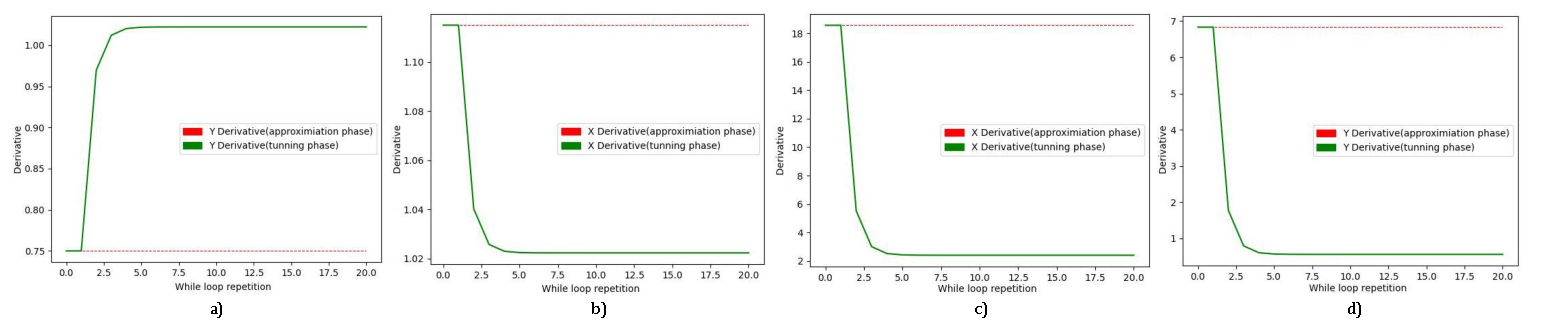
\includegraphics[width=\textwidth]{charts.pdf}
	\caption{Estimated derivative for $e^{(x+y)}$ function from: a) the proposed method I for the noise-free scenario, b) the proposed method III for the noise-free scenario, c) the proposed method I for the noisy version of this function in the original point $(0,0)$, and d) the proposed method III for the noisy version of this function in the original point $(0,0)$.}
	\label{3D_cur23}
\end{figure}

The derivative at the reference point $(0,0)$ is first computed using the proposed methods prior to any parameter tuning. The results for the noise-free case are presented in Fig.~\ref{3D_cur23}(a) and (b). As observed, both methods exhibit fast convergence toward the exact derivative value, indicating the correctness of the underlying mathematical formulation.
\FloatBarrier

To further evaluate robustness, Gaussian noise with a signal-to-noise ratio (SNR) of 10 dB is added to the synthetic function. The corresponding results are shown in Fig.~\ref{3D_cur23}(c) and (d). Despite the presence of noise, the proposed methods are still able to approximate the true derivative with high accuracy, demonstrating strong robustness against noise perturbations.

From a theoretical perspective, it is expected that Methods II and III provide improved performance in noisy conditions compared to Method I, due to their enhanced formulation. In particular, Method III is anticipated to be more robust against impulsive disturbances and outliers, such as salt-and-pepper noise.

%------------------------------------------------
\FloatBarrier
\subsection{Parameter Analysis of the Proposed Methods}
This subsection investigates the influence of key parameters on the performance of the proposed methods and aims to determine suitable parameter settings for subsequent experiments. In particular, the effects of the neighborhood size $n$ and the step parameter $h$ are analyzed under both noise-free and noisy conditions. Furthermore, the computational complexity of the proposed methods is evaluated.

fig. \ref{New2} shows a comparison of the corresponding outputs with different $n$ and $h$, indicating the number of expressions and the unit distance between the two processed points in the image for the proposed method I, II, and III.

\FloatBarrier
\begin{figure}[H]
	\centering
	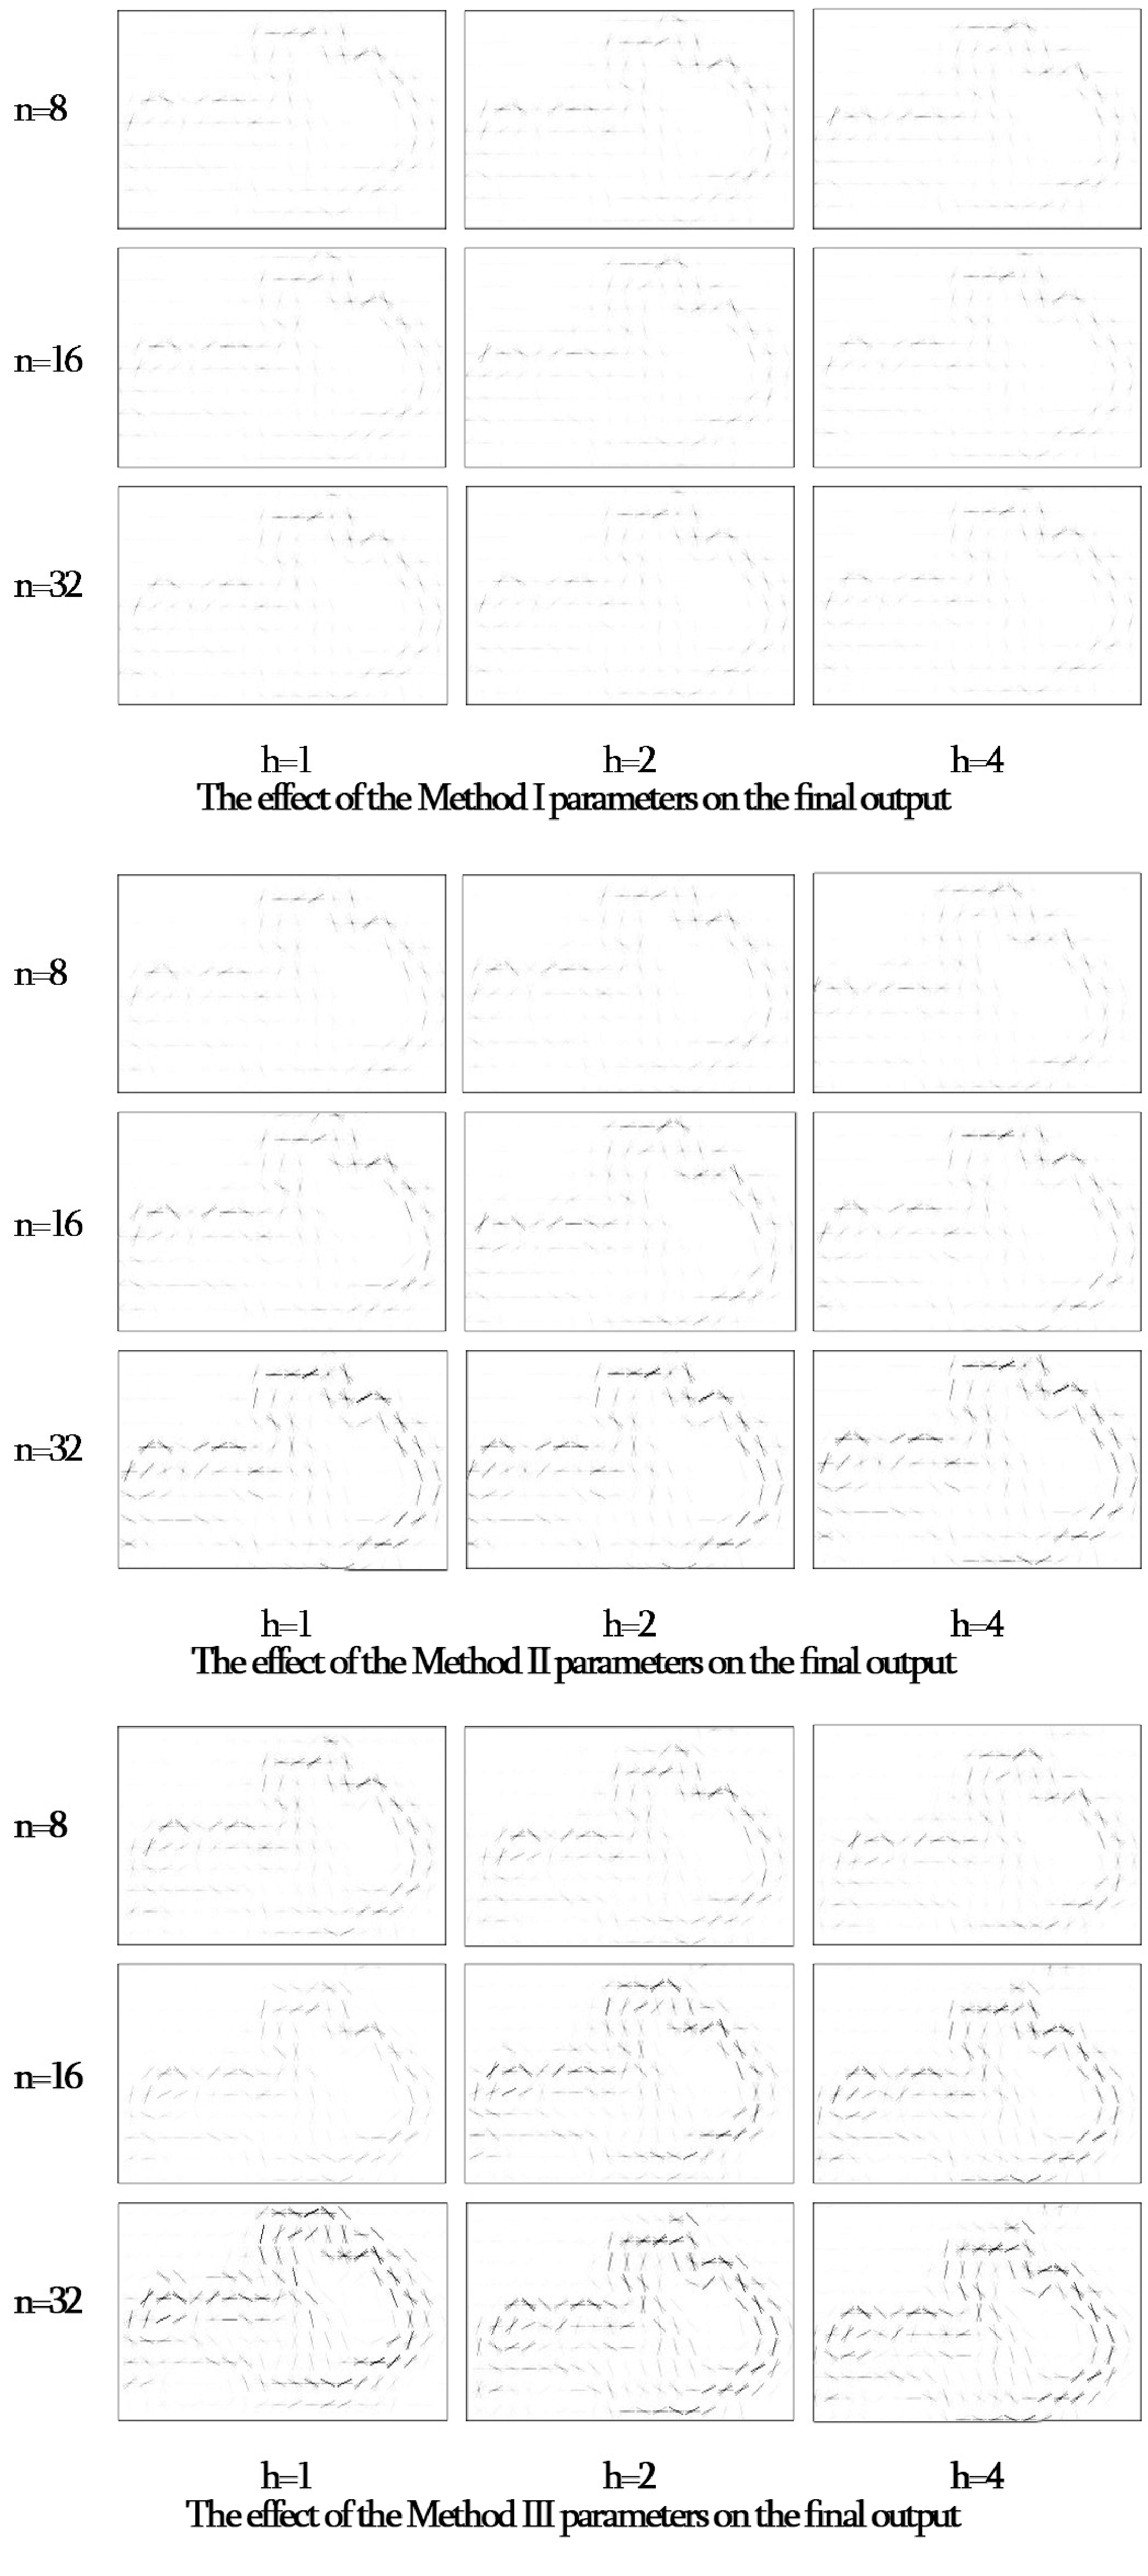
\includegraphics[width=\textwidth]{allInOne.pdf}
	\caption{Comparing the intensity of recognized edges for proposed method I, II, and III over different $h$ and $n$.}
	\label{New2}
\end{figure}
\FloatBarrier

%-------------------------------------------

To show the strength of these two proposed algorithms, we designed a new experiment to compare them with the proposed method I.
In this experiment, we synthetically got stained the images with noise with different powers, i.e., 25 dB and 50 dB for Gaussian noise, and 3\% and 5\% for salt and pepper noise.
We repeated the experiments for different images and different noise powers.
We also examined the effect of two variables $n=5,8,16$ and $h=1,2$.
Table \ref{tab4} summarizes these results for cameraman image.
According to these results, the proposed methods II and III in particular to eliminate the effect of salt and pepper noise are well visible.
Also, for high percentages of this noise, the proposed method III works better than the proposed method II.
For example, in $n=16$, $h=2$, with the 5\% salt and pepper noise, the output of the proposed method III is better than the outputs of the proposed method I and III. 

%------------------------------------------------

\begin{table}[!h]
	\centering
	\caption{Investigating the effect of three parameters, i.e., $n=5,8,16$, $h=1,2$ , and noise power on the performance of the proposed methods I, II and III, for cameraman image}
	\label{tab4}
	\begin{adjustbox}{width=14cm,height=11.8cm}
		
		\begin{tabular}{llllcccc}
			\hline
			n & Noise type & Power & h & \multicolumn{1}{l}{Input} & \multicolumn{1}{l}{\begin{tabular}[c]{@{}l@{}}Proposed\\ method I\end{tabular}} & \multicolumn{1}{l}{\begin{tabular}[c]{@{}l@{}}Proposed\\ method II\end{tabular}} & \begin{tabular}[c]{@{}c@{}}proposed\\ method III\end{tabular} \\ \hline
			%-------------------------------------------------------------------
			\multirow{22}{*}{5} & \multirow{8}{*}{Gaussian}
			& 25 dB & \multirow{2}{*}{1}
			& 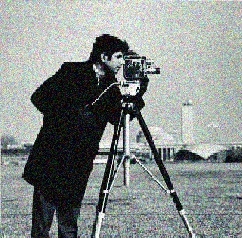
\includegraphics[width=1in,height=1in]{cameraman_gaussian25_T4_i1.jpg}
			&
\includegraphics[width=1in,height=1in]{bigtable-seri3/noise_25_h_1_n_4.jpg}
			&
\includegraphics[width=1in,height=1in]{bigtable-seri2/noise_25_h_1_n_4.jpg}
			&
\includegraphics[width=1in,height=1in]{bigtable-seri3/noise_25_h_1_n_4.jpg}
			\\ \cline{3-3} \cline{5-8} 
			&  & 50 dB &  
			&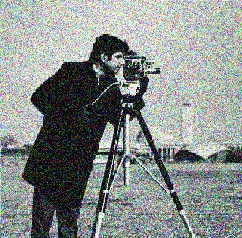
\includegraphics[width=1in,height=1in]{cameraman_gaussian50_T4_i1.jpg}
			&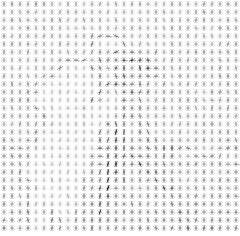
\includegraphics[width=1in,height=1in]{bigtable-seri1/noise_50_h_1_n_4.jpg}
			&
\includegraphics[width=1in,height=1in]{bigtable-seri2/noise_50_h_1_n_4.jpg}
			&
\includegraphics[width=1in,height=1in]{bigtable-seri3/noise_50_h_1_n_4.jpg}
			\\ \cline{3-8} 
			&  & 25 dB & \multirow{2}{*}{2}
			& 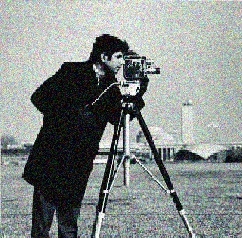
\includegraphics[width=1in,height=1in]{cameraman_gaussian25_T4_i1.jpg}
			& 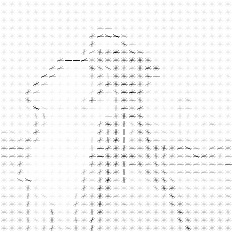
\includegraphics[width=1in,height=1in]{bigtable-seri1/noise_25_h_2_n_4.jpg}
			&
\includegraphics[width=1in,height=1in]{bigtable-seri2/noise_25_h_2_n_4.jpg}
			&
\includegraphics[width=1in,height=1in]{bigtable-seri3/noise_25_h_2_n_4.jpg}
			\\ \cline{3-3} \cline{5-8} 
			&  & 50 dB & 
			&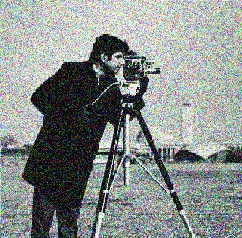
\includegraphics[width=1in,height=1in]{cameraman_gaussian50_T4_i1.jpg}
			&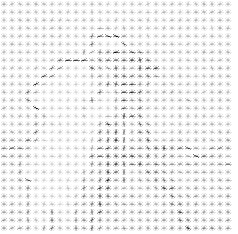
\includegraphics[width=1in,height=1in]{bigtable-seri1/noise_50_h_2_n_4.jpg}
			&
\includegraphics[width=1in,height=1in]{bigtable-seri2/noise_50_h_2_n_4.jpg}
			&
\includegraphics[width=1in,height=1in]{bigtable-seri3/noise_50_h_2_n_4.jpg}
			\\ \cline{2-8} 
			& \multirow{8}{*}{Salt and pepper} & 3 $\%$ & \multirow{2}{*}{1}
			& 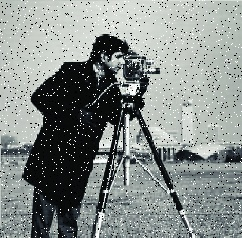
\includegraphics[width=1in,height=1in]{cameraman_salt3_T4_i1.jpg}
			& 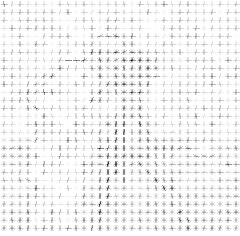
\includegraphics[width=1in,height=1in]{bigtable-seri1/noise_3_h_1_n_4.jpg}
			&
\includegraphics[width=1in,height=1in]{bigtable-seri2/noise_3_h_1_n_4.jpg}
			&
\includegraphics[width=1in,height=1in]{bigtable-seri3/noise_3_h_1_n_4.jpg}
			\\ \cline{3-3} \cline{5-8} 
			&  & 5 $\%$ & 
			& 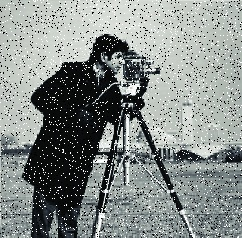
\includegraphics[width=1in,height=1in]{cameraman_salt5_T4_i1.jpg}
			&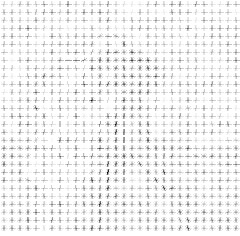
\includegraphics[width=1in,height=1in]{bigtable-seri1/noise_5_h_1_n_4.jpg}
			&
\includegraphics[width=1in,height=1in]{bigtable-seri2/noise_5_h_1_n_4.jpg}
			&
\includegraphics[width=1in,height=1in]{bigtable-seri3/noise_5_h_1_n_4.jpg}
			\\ \cline{3-8} 
			&  & 3 $\%$ & \multirow{2}{*}{2}
			& 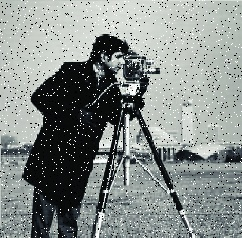
\includegraphics[width=1in,height=1in]{cameraman_salt3_T4_i1.jpg}
			&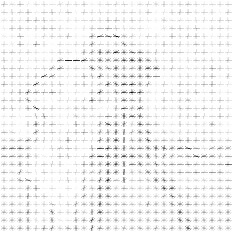
\includegraphics[width=1in,height=1in]{bigtable-seri1/noise_3_h_2_n_4.jpg}
			&
\includegraphics[width=1in,height=1in]{bigtable-seri2/noise_3_h_2_n_4.jpg}
			&
\includegraphics[width=1in,height=1in]{bigtable-seri3/noise_3_h_2_n_4.jpg}
			\\ \cline{3-3} \cline{5-8} 
			&  & 5 $\%$ &
			& 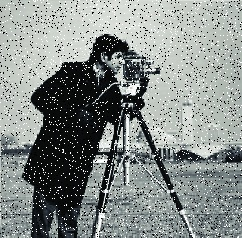
\includegraphics[width=1in,height=1in]{cameraman_salt5_T4_i1.jpg}
			& 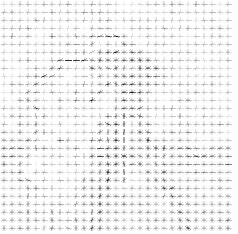
\includegraphics[width=1in,height=1in]{bigtable-seri1/noise_5_h_2_n_4.jpg}
			& 
\includegraphics[width=1in,height=1in]{bigtable-seri2/noise_5_h_2_n_4.jpg}
			& 
\includegraphics[width=1in,height=1in]{bigtable-seri3/noise_5_h_2_n_4.jpg}
			\\ \hline
			%-------------------------------------------------------------------
			
			\multirow{22}{*}{8} & \multirow{8}{*}{Gaussian}
			& 25 dB & \multirow{2}{*}{1}
			& 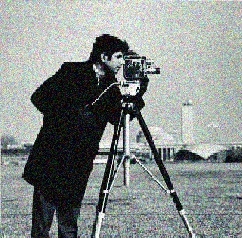
\includegraphics[width=1in,height=1in]{cameraman_gaussian25_T4_i1.jpg}
			&
\includegraphics[width=1in,height=1in]{bigtable-seri3/noise_25_h_1_n_8.jpg}
			&
\includegraphics[width=1in,height=1in]{bigtable-seri2/noise_25_h_1_n_8.jpg}
			&
\includegraphics[width=1in,height=1in]{bigtable-seri3/noise_25_h_1_n_8.jpg}
			\\ \cline{3-3} \cline{5-8} 
			&  & 50 dB &  
			&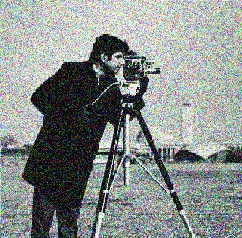
\includegraphics[width=1in,height=1in]{cameraman_gaussian50_T4_i1.jpg}
			&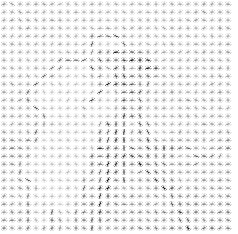
\includegraphics[width=1in,height=1in]{bigtable-seri1/noise_50_h_1_n_8.jpg}
			&
\includegraphics[width=1in,height=1in]{bigtable-seri2/noise_50_h_1_n_8.jpg}
			&
\includegraphics[width=1in,height=1in]{bigtable-seri3/noise_50_h_1_n_8.jpg}
			\\ \cline{3-8} 
			&  & 25 dB & \multirow{2}{*}{2}
			& 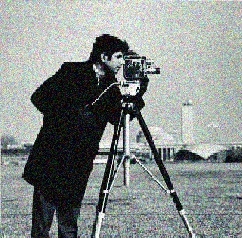
\includegraphics[width=1in,height=1in]{cameraman_gaussian25_T4_i1.jpg}
			& 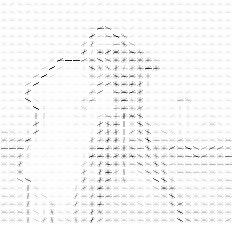
\includegraphics[width=1in,height=1in]{bigtable-seri1/noise_25_h_2_n_8.jpg}
			&
\includegraphics[width=1in,height=1in]{bigtable-seri2/noise_25_h_2_n_8.jpg}
			&
\includegraphics[width=1in,height=1in]{bigtable-seri3/noise_25_h_2_n_8.jpg}
			\\ \cline{3-3} \cline{5-8} 
			&  & 50 dB & 
			&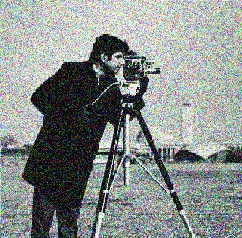
\includegraphics[width=1in,height=1in]{cameraman_gaussian50_T4_i1.jpg}
			&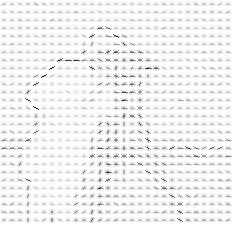
\includegraphics[width=1in,height=1in]{bigtable-seri1/noise_50_h_2_n_8.jpg}
			&
\includegraphics[width=1in,height=1in]{bigtable-seri2/noise_50_h_2_n_8.jpg}
			&
\includegraphics[width=1in,height=1in]{bigtable-seri3/noise_50_h_2_n_8.jpg}
			\\ \cline{2-8} 
			& \multirow{8}{*}{Salt and pepper} & 3 $\%$ & \multirow{2}{*}{1}
			& 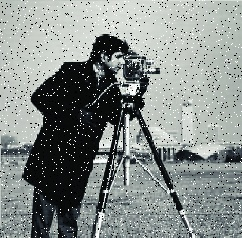
\includegraphics[width=1in,height=1in]{cameraman_salt3_T4_i1.jpg}
			& 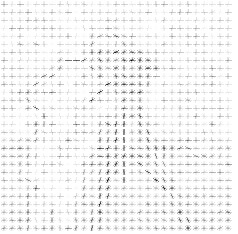
\includegraphics[width=1in,height=1in]{bigtable-seri1/noise_3_h_1_n_8.jpg}
			&
\includegraphics[width=1in,height=1in]{bigtable-seri2/noise_3_h_1_n_8.jpg}
			&
\includegraphics[width=1in,height=1in]{bigtable-seri3/noise_3_h_1_n_8.jpg}
			\\ \cline{3-3} \cline{5-8} 
			&  & 5 $\%$ & 
			& 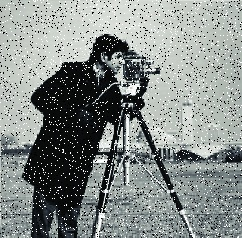
\includegraphics[width=1in,height=1in]{cameraman_salt5_T4_i1.jpg}
			&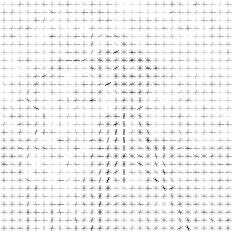
\includegraphics[width=1in,height=1in]{bigtable-seri1/noise_5_h_1_n_8.jpg}
			&
\includegraphics[width=1in,height=1in]{bigtable-seri2/noise_5_h_1_n_8.jpg}
			&
\includegraphics[width=1in,height=1in]{bigtable-seri3/noise_5_h_1_n_8.jpg}
			\\ \cline{3-8} 
			&  & 3 $\%$ & \multirow{2}{*}{2}
			& 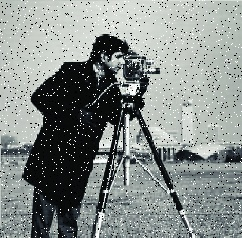
\includegraphics[width=1in,height=1in]{cameraman_salt3_T4_i1.jpg}
			&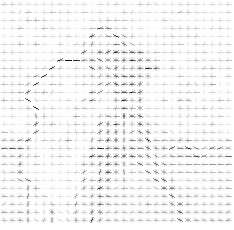
\includegraphics[width=1in,height=1in]{bigtable-seri1/noise_3_h_2_n_8.jpg}
			&
\includegraphics[width=1in,height=1in]{bigtable-seri2/noise_3_h_2_n_8.jpg}
			&
\includegraphics[width=1in,height=1in]{bigtable-seri3/noise_3_h_2_n_8.jpg}
			\\ \cline{3-3} \cline{5-8} 
			&  & 5 $\%$ &
			& 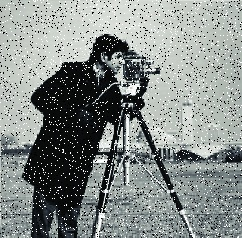
\includegraphics[width=1in,height=1in]{cameraman_salt5_T4_i1.jpg}
			& 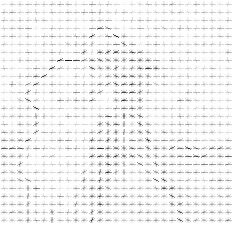
\includegraphics[width=1in,height=1in]{bigtable-seri1/noise_5_h_2_n_8.jpg}
			& 
\includegraphics[width=1in,height=1in]{bigtable-seri2/noise_5_h_2_n_8.jpg}
			& 
\includegraphics[width=1in,height=1in]{bigtable-seri3/noise_5_h_2_n_8.jpg}
			\\ \hline
			%-------------------------------------------------------------------
			
			%-------------------------------------------------------------------
		\end{tabular}
	\end{adjustbox}
\end{table}

\begin{table}[!h]
	\begin{adjustbox}{width=14cm,height=5.9cm}
		\begin{tabular}{llllcccc}
			\multirow{22}{*}{16} & \multirow{8}{*}{Gaussian}
			& 25 dB & \multirow{2}{*}{1}
			& 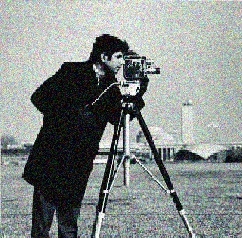
\includegraphics[width=1in,height=1in]{cameraman_gaussian25_T4_i1.jpg}
			&
\includegraphics[width=1in,height=1in]{bigtable-seri3/noise_25_h_1_n_16.jpg}
			&
\includegraphics[width=1in,height=1in]{bigtable-seri2/noise_25_h_1_n_16.jpg}
			&
\includegraphics[width=1in,height=1in]{bigtable-seri3/noise_25_h_1_n_16.jpg}
			\\ \cline{3-3} \cline{5-8} 
			&  & 50 dB &  
			&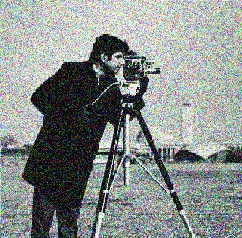
\includegraphics[width=1in,height=1in]{cameraman_gaussian50_T4_i1.jpg}
			&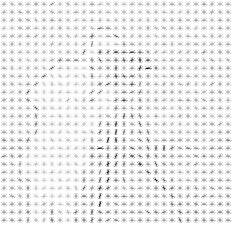
\includegraphics[width=1in,height=1in]{bigtable-seri1/noise_50_h_1_n_16.jpg}
			&
\includegraphics[width=1in,height=1in]{bigtable-seri2/noise_50_h_1_n_16.jpg}
			&
\includegraphics[width=1in,height=1in]{bigtable-seri3/noise_50_h_1_n_16.jpg}
			\\ \cline{3-8} 
			&  & 25 dB & \multirow{2}{*}{2}
			& 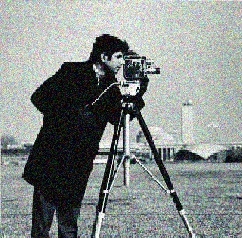
\includegraphics[width=1in,height=1in]{cameraman_gaussian25_T4_i1.jpg}
			& 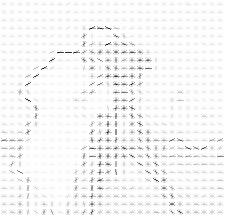
\includegraphics[width=1in,height=1in]{bigtable-seri1/noise_25_h_2_n_16.jpg}
			&
\includegraphics[width=1in,height=1in]{bigtable-seri2/noise_25_h_2_n_16.jpg}
			&
\includegraphics[width=1in,height=1in]{bigtable-seri3/noise_25_h_2_n_16.jpg}
			\\ \cline{3-3} \cline{5-8} 
			&  & 50 dB & 
			&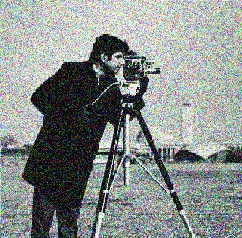
\includegraphics[width=1in,height=1in]{cameraman_gaussian50_T4_i1.jpg}
			&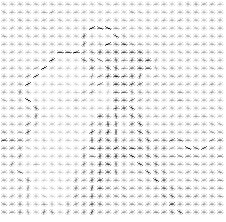
\includegraphics[width=1in,height=1in]{bigtable-seri1/noise_50_h_2_n_16.jpg}
			&
\includegraphics[width=1in,height=1in]{bigtable-seri2/noise_50_h_2_n_16.jpg}
			&
\includegraphics[width=1in,height=1in]{bigtable-seri3/noise_50_h_2_n_16.jpg}
			\\ \cline{2-8} 
			& \multirow{8}{*}{Salt and pepper} & 3 $\%$ & \multirow{2}{*}{1}
			& 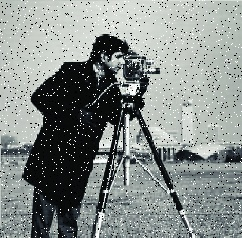
\includegraphics[width=1in,height=1in]{cameraman_salt3_T4_i1.jpg}
			& 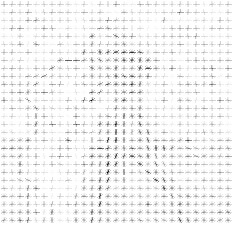
\includegraphics[width=1in,height=1in]{bigtable-seri1/noise_3_h_1_n_16.jpg}
			&
\includegraphics[width=1in,height=1in]{bigtable-seri2/noise_3_h_1_n_16.jpg}
			&
\includegraphics[width=1in,height=1in]{bigtable-seri3/noise_3_h_1_n_16.jpg}
			\\ \cline{3-3} \cline{5-8} 
			&  & 5 $\%$ & 
			& 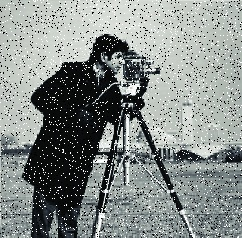
\includegraphics[width=1in,height=1in]{cameraman_salt5_T4_i1.jpg}
			&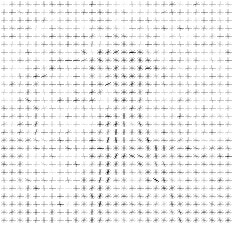
\includegraphics[width=1in,height=1in]{bigtable-seri1/noise_5_h_1_n_16.jpg}
			&
\includegraphics[width=1in,height=1in]{bigtable-seri2/noise_5_h_1_n_16.jpg}
			&
\includegraphics[width=1in,height=1in]{bigtable-seri3/noise_5_h_1_n_16.jpg}
			\\ \cline{3-8} 
			&  & 3 $\%$ & \multirow{2}{*}{2}
			& 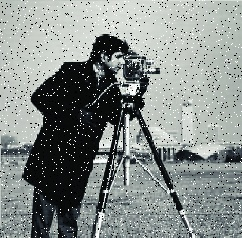
\includegraphics[width=1in,height=1in]{cameraman_salt3_T4_i1.jpg}
			&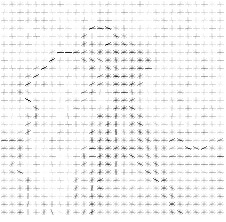
\includegraphics[width=1in,height=1in]{bigtable-seri1/noise_3_h_2_n_16.jpg}
			&
\includegraphics[width=1in,height=1in]{bigtable-seri2/noise_3_h_2_n_16.jpg}
			&
\includegraphics[width=1in,height=1in]{bigtable-seri3/noise_3_h_2_n_16.jpg}
			\\ \cline{3-3} \cline{5-8} 
			&  & 5 $\%$ &
			& 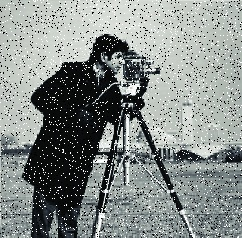
\includegraphics[width=1in,height=1in]{cameraman_salt5_T4_i1.jpg}
			& 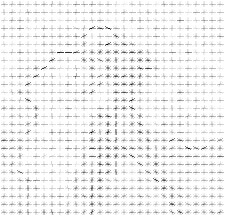
\includegraphics[width=1in,height=1in]{bigtable-seri1/noise_5_h_2_n_16.jpg}
			& 
\includegraphics[width=1in,height=1in]{bigtable-seri2/noise_5_h_2_n_16.jpg}
			& 
\includegraphics[width=1in,height=1in]{bigtable-seri3/noise_5_h_2_n_16.jpg}
		\end{tabular}
	\end{adjustbox}
\end{table}
%------------------------------------------------

Figs. \ref{fig7_1} and \ref{fig7_2} show the outputs of the three proposed methods I,II, and III for $n = 16$, $h = 1$ over noise-free images. According to these results, HOGs for seven images \footnote{http://pascal.inrialpes.fr/data} are extracted which are from different scenes.
These results are extracted for noise-free and clear images, and the inverted of them are finally presented.
%As can be seen, the proposed method I has extracted the edge lines well, but in some areas, these lines are very faint and weak.
The proposed methods I and II extracted the edge lines of the objects in the image scenes, but as can be seen, the performances of these methods are close to each other in this concept.
It is noticeable that because of optimizing the sum of derivatives, 
the total derivative amounts are stronger in the proposed methods II and III (as reveals in the second picture in fig. \ref{fig7_1}). We should mention that the points used in the method II and III are different from the points used in approximation phase. It is because we focus on gaining the first two derivatives in the first method while we ignore the remained terms by placing particular points into the system (but the main concentration is noise reduction in the method II and III).
For this reason, although the edges are more solid in some points in method II and III, the directions of the image HOG in that points are destroyed.  
%Besides, the performance of the last two proposed methods is almost the same in this concept.

%-----------------------------------------------------------
\begin{figure*}[!h]
	\centering
	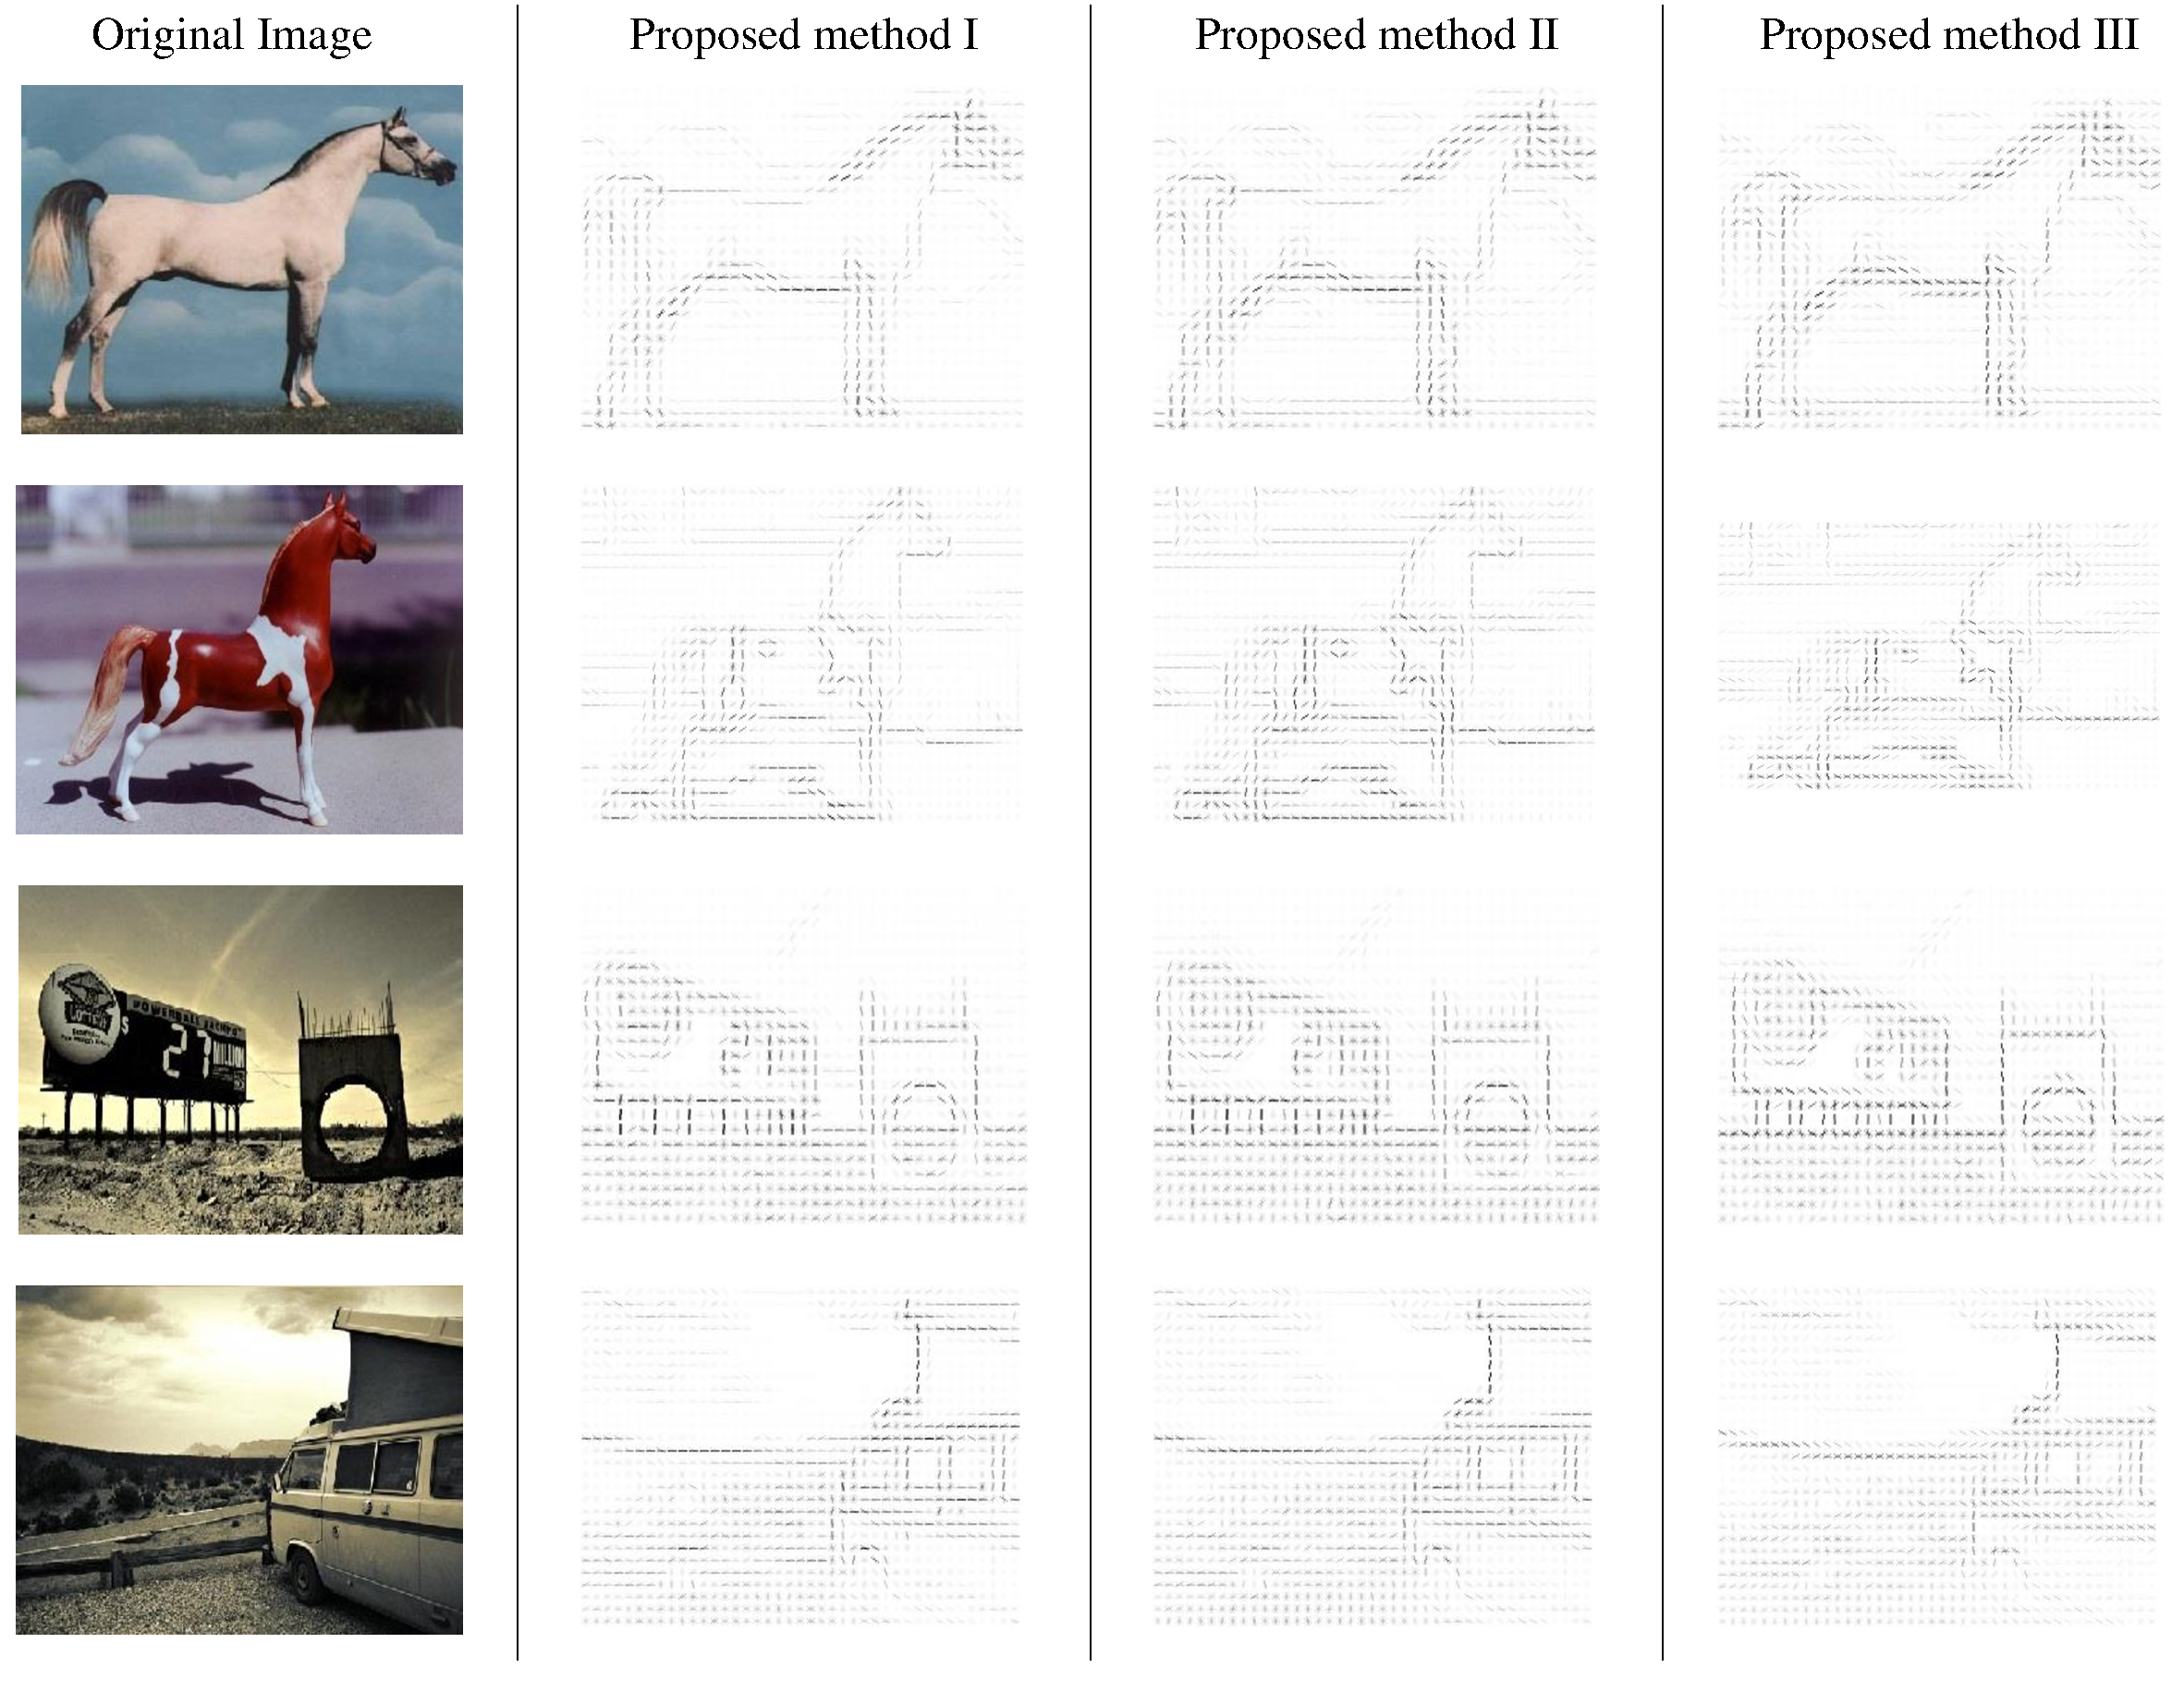
\includegraphics[height=8.0cm,width=12cm]{fig6_new.pdf}
	\caption{HOG results for four pictures using proposed methods I, II, and III.}
	\label{fig7_1}
\end{figure*}


\begin{figure*}[!h]
	\centering
	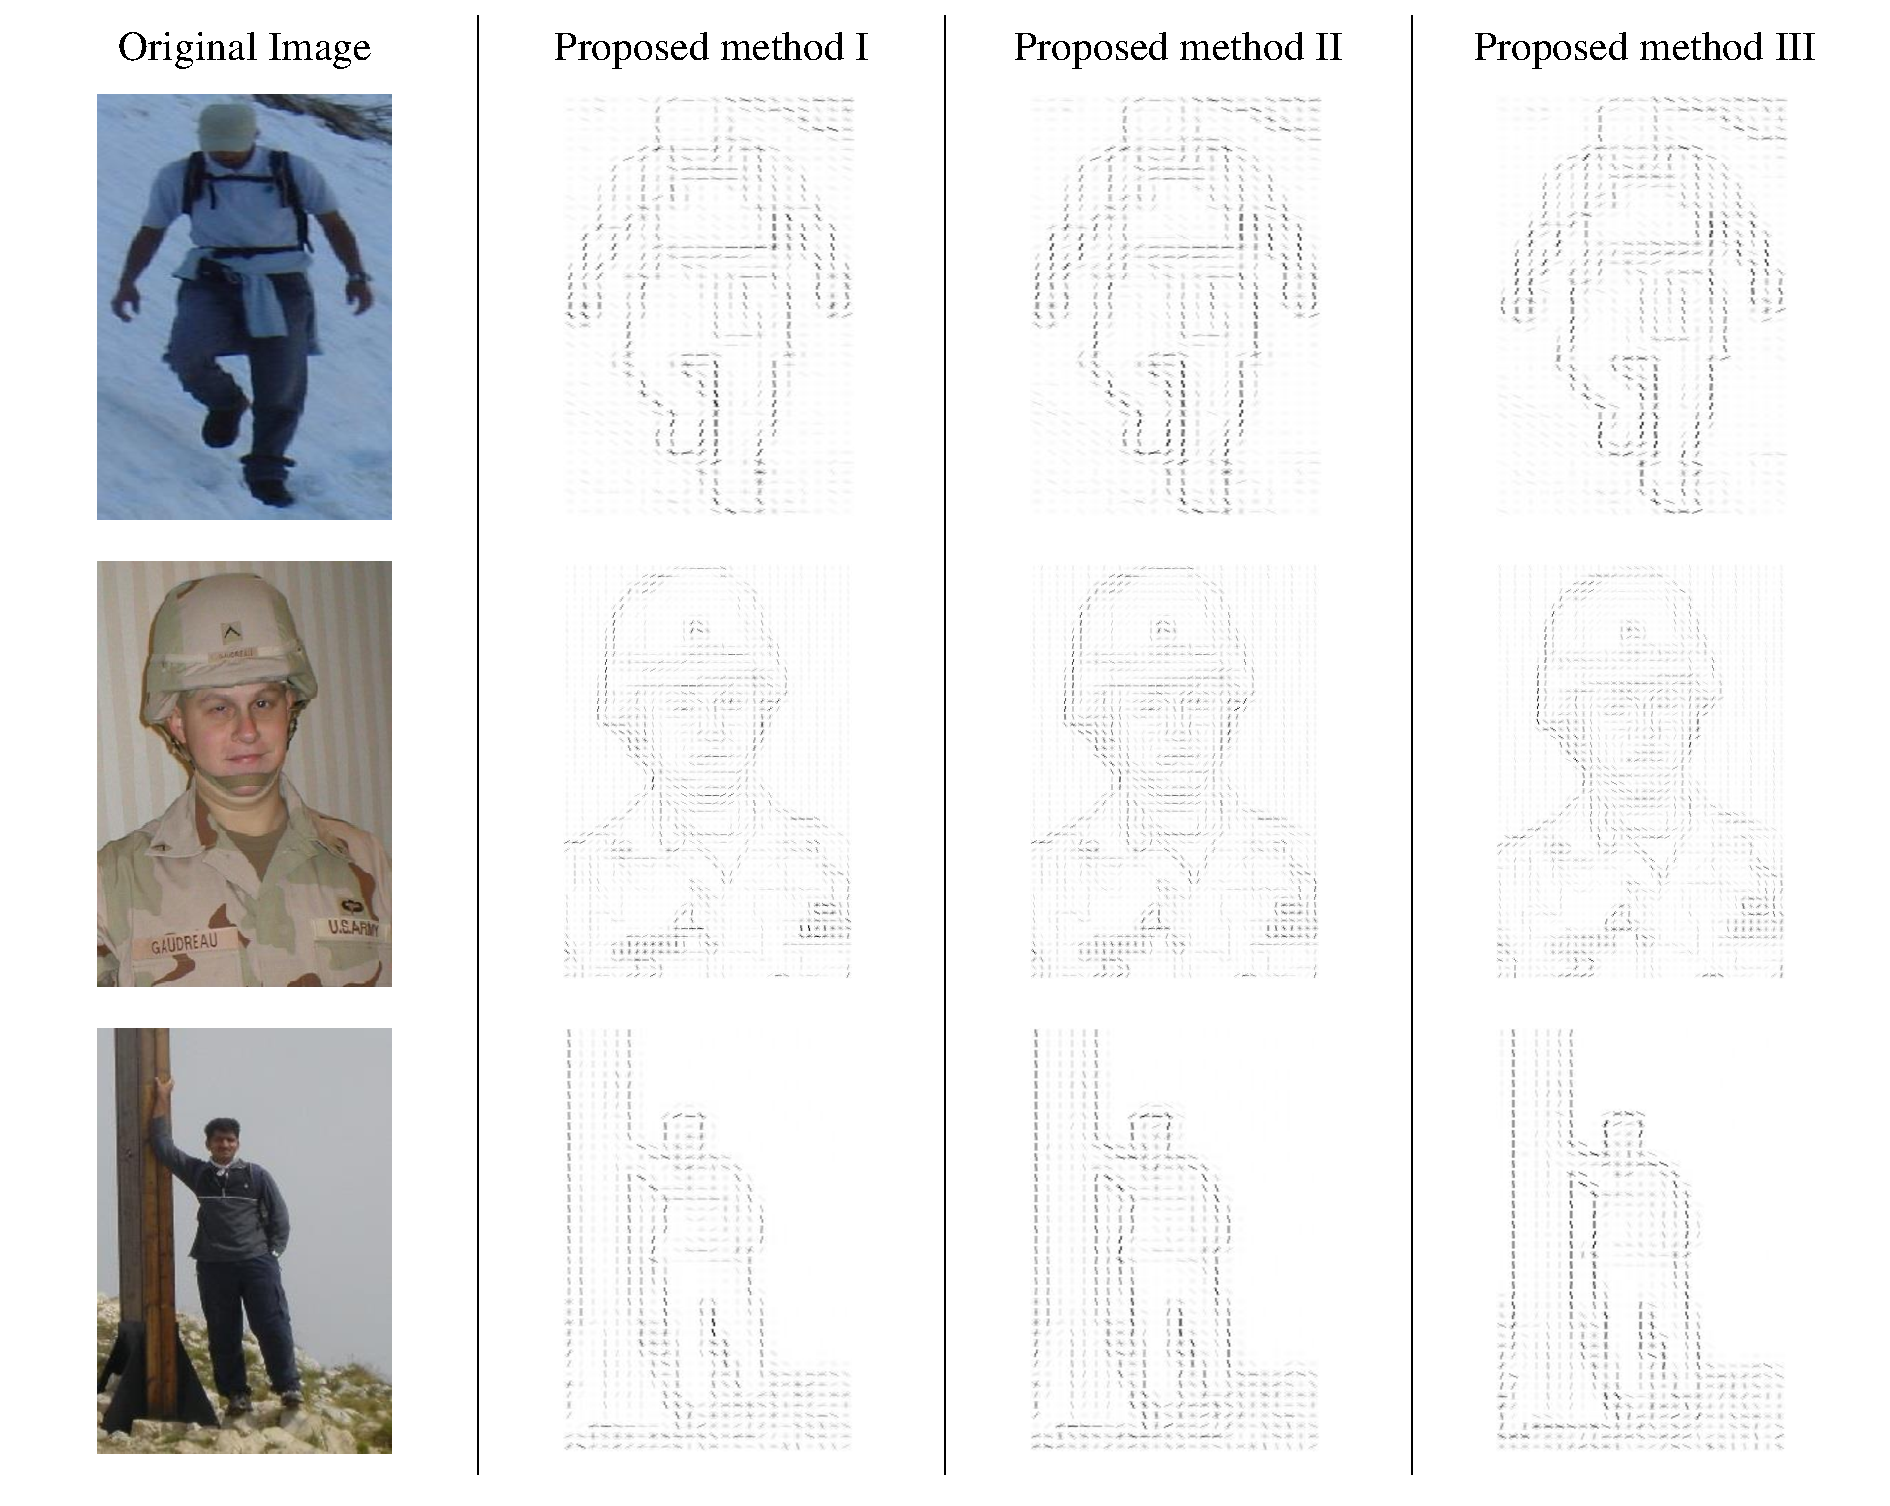
\includegraphics[height=8.0cm,width=12cm]{fig7_new.pdf}
	\caption{HOG results for three pictures proposed methods I, II, and III.}
	\label{fig7_2}
\end{figure*}
%----------------------------------------------------------

As shown in fig. \ref{fig7_122}, we obtained the outputs of the proposed methods I and III over two images contaminated by $5\%$ salt and pepper noise. The output of the proposed method I is acceptable by comparing with Sobel method in the experiments. Also, we should mention that the final result can be better by adjusting the larger matrix size. However, there is a much more clear image than this result provided from the proposed method III in the sub-fig. b), in which the edges are almost as clear as a noisy-less image. Obviously, the influence of noise on this image approximately disappeared.
%-----------------------------------------------------------
\FloatBarrier
\begin{figure*}[!th]
	\centering
	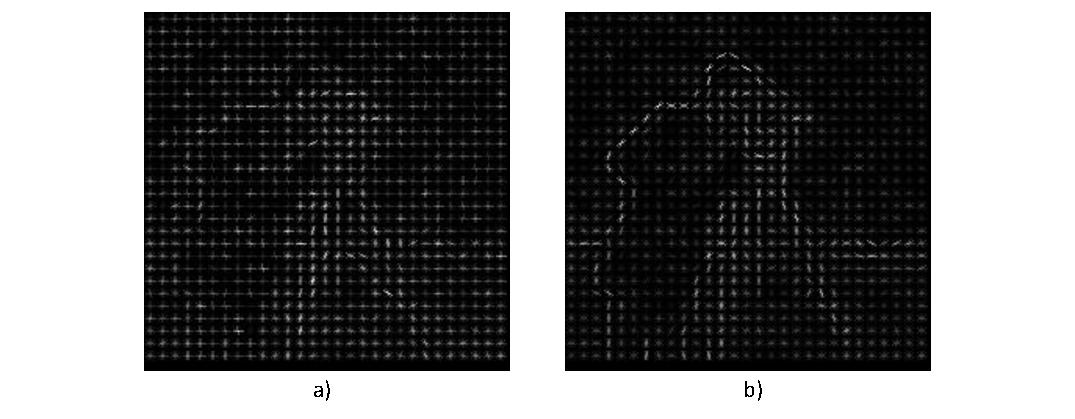
\includegraphics[height=4.0cm,width=12.25cm]{first_analyze.pdf}
	\caption{The outputs of the proposed methods I and III for the one noisy picture.}
	\label{fig7_122}
\end{figure*}
%-----------------------------------------------------------

Three-dimensional bar charts are plotted in fig. \ref{3D_cur} to analyze the effects of various sizes of the images and $n$ on the total run-time for the proposed method I, II, and III.
As can be seen, the proposed methods I has a higher speed on different image sizes and different degrees of derivative.
In addition, the other two proposed methods have almost the same performance in terms of time.
%-----------------------------------------------------------	
\FloatBarrier
\begin{figure*}[!th]
	\centering
	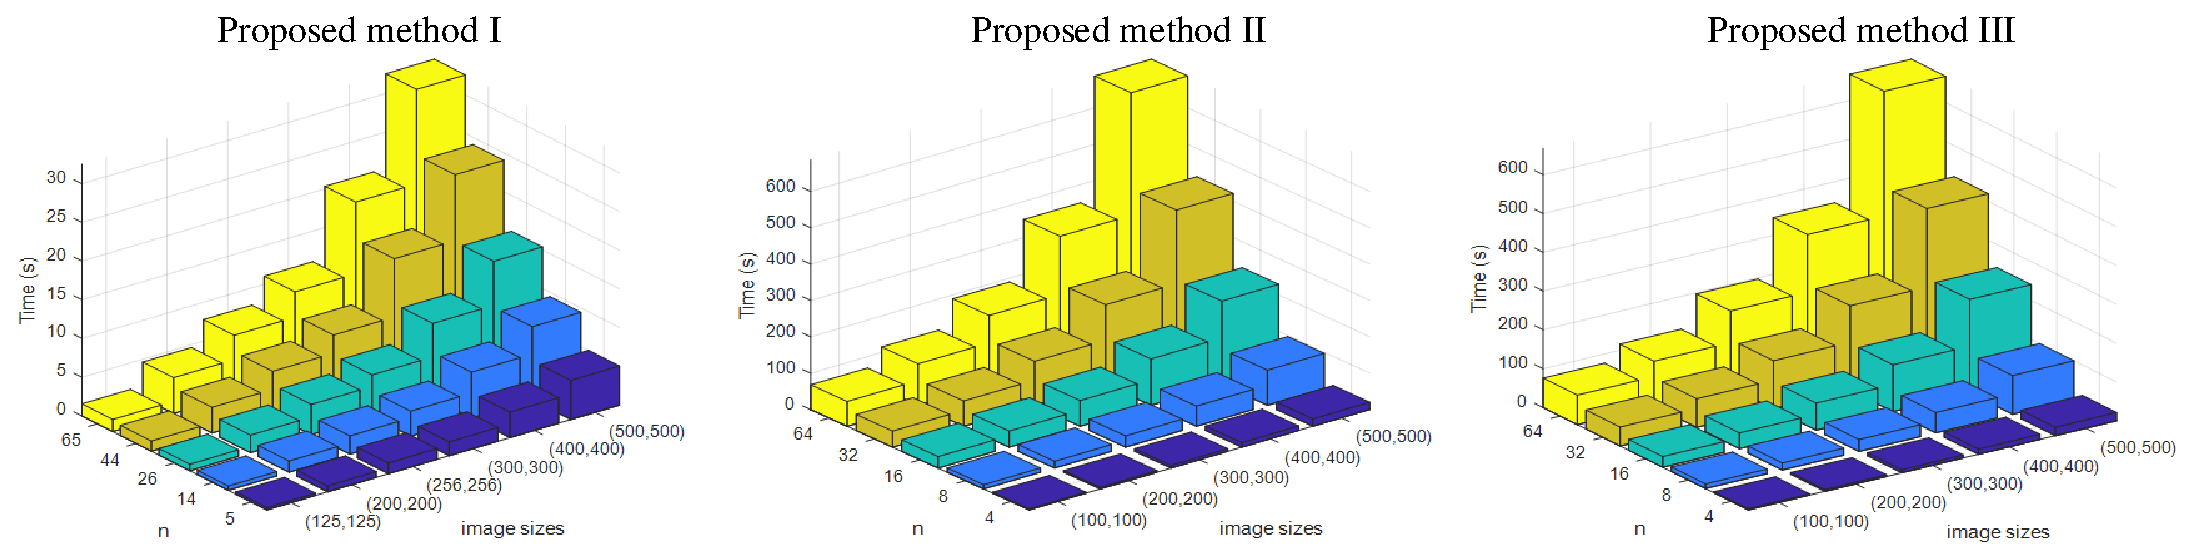
\includegraphics[height=3.1cm,width=15cm]{3D_curves.pdf}
	\caption{The effects of $n$ and image sizes on run time for three proposed methods I, II, and III.}
	\label{3D_cur}
\end{figure*}
%-----------------------------------------------------------


%-----------------------------------------------------------
\subsection{Comparison with Existing Methods}

%------------------------------------------------
\FloatBarrier
\begin{table}[!h]
\centering
\caption{Performance evaluation, for the proposed methods I, II, and III (with $h=1$ and $n=32$) and other compared method, i.e., Sobel over four images without noise}
\label{tab1}
\begin{adjustbox}{width=10cm,height=3.25cm}

\begin{tabular}{l|l|l|l|l}
\hline \hline
\begin{tabular}[c]{@{}l@{}}Original clean\\ image\end{tabular}
& 
\includegraphics[width=0.5in,height=0.5in]{cameraman.png}  
& 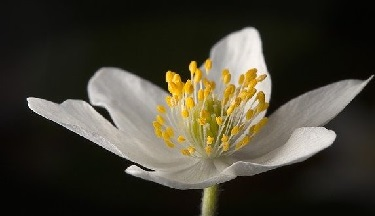
\includegraphics[width=0.5in,height=0.5in]{flower.jpg}
& 
\includegraphics[width=0.5in,height=0.5in]{girl.png}
& 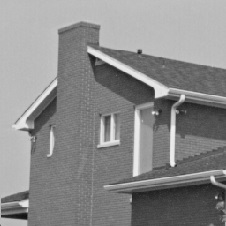
\includegraphics[width=0.5in,height=0.5in]{home.jpg}
\\ \hline

\begin{tabular}[c]{@{}l@{}}Proposed Method I\end{tabular} 
& 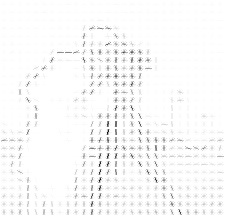
\includegraphics[width=0.5in,height=0.5in]{second_table_n0_s1/cnoise_0.jpg}
& 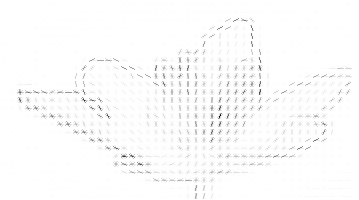
\includegraphics[width=0.5in,height=0.5in]{second_table_n0_s1/fnoise_0.jpg}
& 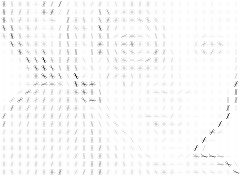
\includegraphics[width=0.5in,height=0.5in]{second_table_n0_s1/gnoise_0.jpg}
& 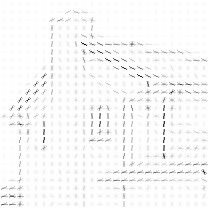
\includegraphics[width=0.5in,height=0.5in]{second_table_n0_s1/hnoise_0.jpg}
\\ \hline

\begin{tabular}[c]{@{}l@{}}Proposed Method II\end{tabular} 
& 
\includegraphics[width=0.5in,height=0.5in]{second_table_n0_s2/cnoise_0.jpg}
& 
\includegraphics[width=0.5in,height=0.5in]{second_table_n0_s2/fnoise_0.jpg} 
& 
\includegraphics[width=0.5in,height=0.5in]{second_table_n0_s2/gnoise_0.jpg}% size?
& 
\includegraphics[width=0.5in,height=0.5in]{second_table_n0_s2/hnoise_0.jpg}
\\ \hline
%done%done%done%done%done
\begin{tabular}[c]{@{}l@{}}Proposed Method III\end{tabular} 
& 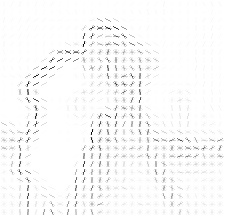
\includegraphics[width=0.5in,height=0.5in]{second_table_n0_s3/cnoise_50.jpg}
& 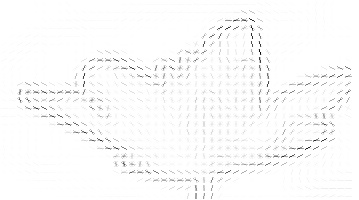
\includegraphics[width=0.5in,height=0.5in]{second_table_n0_s3/fnoise_50.jpg}
& 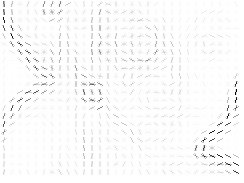
\includegraphics[width=0.5in,height=0.5in]{second_table_n0_s3/gnoise_50.jpg}
& 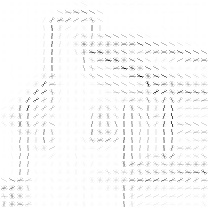
\includegraphics[width=0.5in,height=0.5in]{second_table_n0_s3/hnoise_50.jpg}
\\ \hline

Sobel method
      & 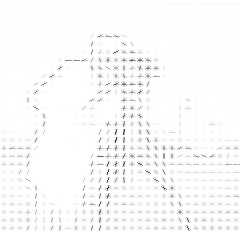
\includegraphics[width=0.5in,height=0.5in]{second_table_sobel_n0/cnoise.jpg}
& 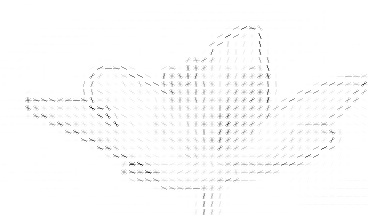
\includegraphics[width=0.5in,height=0.5in]{second_table_sobel_n0/fnoise.jpg}
& 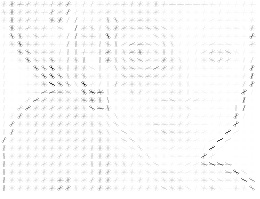
\includegraphics[width=0.5in,height=0.5in]{second_table_sobel_n0/gnoise.jpg}
& 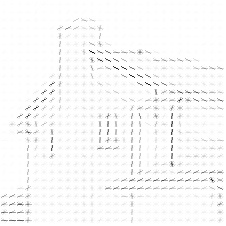
\includegraphics[width=0.5in,height=0.5in]{second_table_sobel_n0/hnoise.jpg}
\\ \hline \hline
\end{tabular}
\end{adjustbox}
\end{table}
%------------------------------------------------
%------------------------------------------------
\begin{table}[!h]
\centering
\caption{Performance evaluation, for the proposed methods I, II, and III (with $h=1$ and $n=32$, respectively) and other compared method, i.e., Sobel over four images contaminated by Gaussian noise with 50$dB$ power}
\label{tab2}
\begin{adjustbox}{width=10cm,height=3.25cm}

\begin{tabular}{l|l|l|l|l}
\hline \hline
\begin{tabular}[c]{@{}l@{}}Noisy image\end{tabular}
    &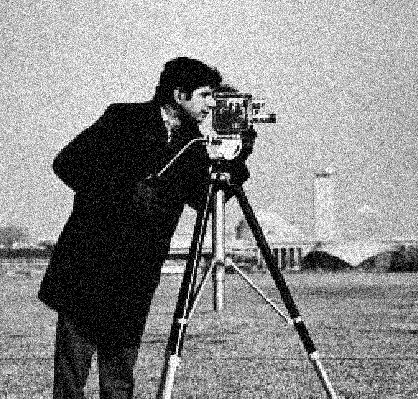
\includegraphics[width=0.5in,height=0.5in]{cameraman_gaussian.jpg}
    &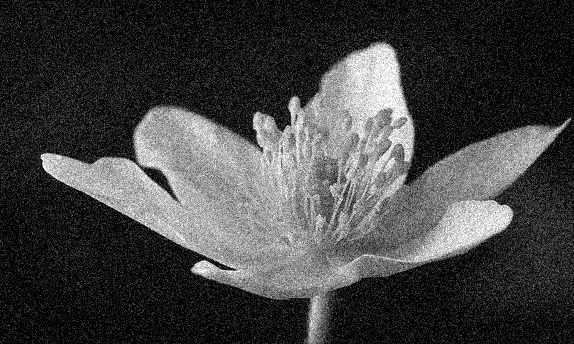
\includegraphics[width=0.5in,height=0.5in]{flower_gussian.jpg}
    &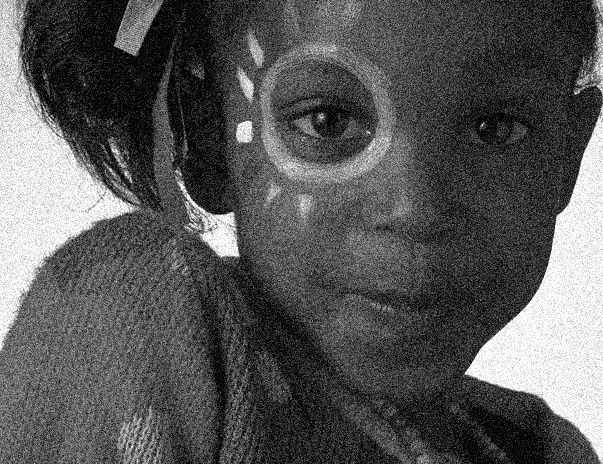
\includegraphics[width=0.5in,height=0.5in]{girl_gaussian.jpg}
    &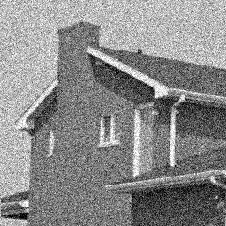
\includegraphics[width=0.5in,height=0.5in]{home_gaussian2.jpg}
\\ \hline
            
\begin{tabular}[c]{@{}l@{}}Proposed Method I\end{tabular} 
& 
\includegraphics[width=0.5in,height=0.5in]{second_table_n50_s1/cnoise_50.jpg}
& 
\includegraphics[width=0.5in,height=0.5in]{second_table_n50_s1/fnoise_50.jpg}
& 
\includegraphics[width=0.5in,height=0.5in]{second_table_n50_s1/gnoise_50.jpg}
& 
\includegraphics[width=0.5in,height=0.5in]{second_table_n50_s1/hnoise_50.jpg}
\\ \hline

\begin{tabular}[c]{@{}l@{}}Proposed Method II\end{tabular} 
& 
\includegraphics[width=0.5in,height=0.5in]{second_table_n50_s2/cnoise_50.jpg}
& 
\includegraphics[width=0.5in,height=0.5in]{second_table_n50_s2/fnoise_50.jpg} 
& 
\includegraphics[width=0.5in,height=0.5in]{second_table_n50_s2/gnoise_50.jpg}% size?
& 
\includegraphics[width=0.5in,height=0.5in]{second_table_n50_s2/hnoise_50.jpg}
\\ \hline
%done%done%done%done%done
\begin{tabular}[c]{@{}l@{}}Proposed Method III\end{tabular} 
& 
\includegraphics[width=0.5in,height=0.5in]{second_table_n50_s3/cnoise_50.jpg}
& 
\includegraphics[width=0.5in,height=0.5in]{second_table_n50_s3/fnoise_50.jpg}
& 
\includegraphics[width=0.5in,height=0.5in]{second_table_n50_s3/gnoise_50.jpg}
& 
\includegraphics[width=0.5in,height=0.5in]{second_table_n50_s3/hnoise_50.jpg}
\\ \hline

Sobel method
& 
\includegraphics[width=0.5in,height=0.5in]{second_table_sobel_n50/cnoise_50.jpg}
& 
\includegraphics[width=0.5in,height=0.5in]{second_table_sobel_n50/fnoise_50.jpg}
& 
\includegraphics[width=0.5in,height=0.5in]{second_table_sobel_n50/gnoise_50.jpg}
& 
\includegraphics[width=0.5in,height=0.5in]{second_table_sobel_n50/hnoise_50.jpg}
\\ \hline \hline        
\end{tabular}
\end{adjustbox}
\end{table}
%------------------------------------------------
%------------------------------------------------
\begin{table}[!th]
\centering
\caption{Performance evaluation, for the proposed methods I, II, and III (with $h=1$ and $n=32$) and other compared method, i.e., Sobel over four images contaminated by 5$\%$ salt and pepper noise }
\label{tab3}
\begin{adjustbox}{width=10cm,height=3.25cm}

\begin{tabular}{l|l|l|l|l}
\hline \hline    
\begin{tabular}[c]{@{}l@{}}Noisy image\end{tabular}
    &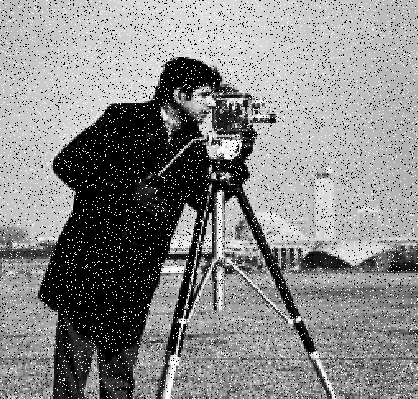
\includegraphics[width=0.5in,height=0.5in]{cameraman_saltpaper.png}
    &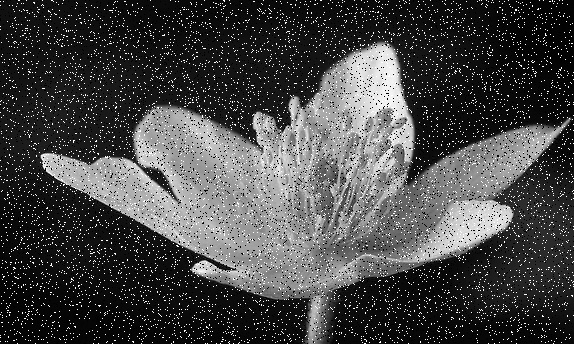
\includegraphics[width=0.5in,height=0.5in]{flower_saltpaper.jpg}   &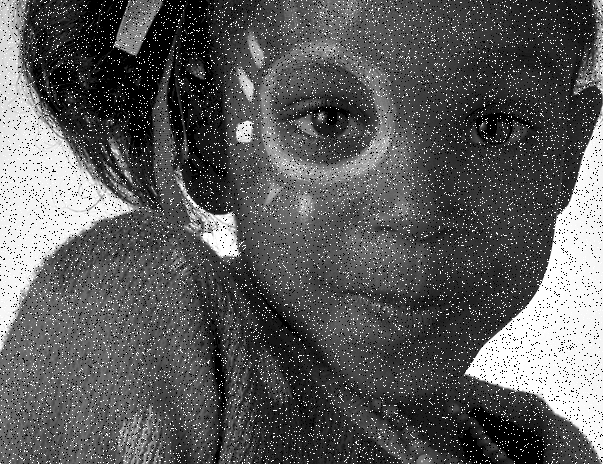
\includegraphics[width=0.5in,height=0.5in]{girl_saltpaper.png}
    &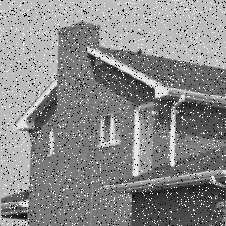
\includegraphics[width=0.5in,height=0.5in]{home_saltpaper_5.png}
\\ \hline

\begin{tabular}[c]{@{}l@{}}Proposed Method I\end{tabular} 
& 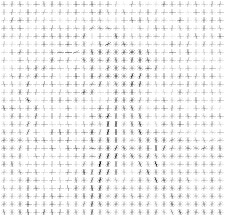
\includegraphics[width=0.5in,height=0.5in]{second_table_n5_s1/cnoise_5.jpg}
& 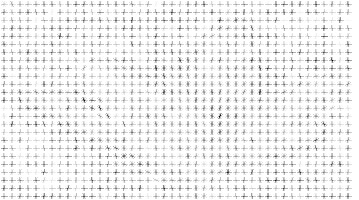
\includegraphics[width=0.5in,height=0.5in]{second_table_n5_s1/fnoise_5.jpg}
& 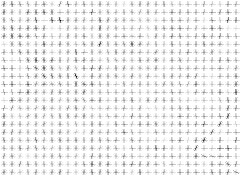
\includegraphics[width=0.5in,height=0.5in]{second_table_n5_s1/gnoise_5.jpg}
& 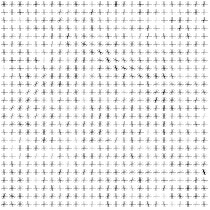
\includegraphics[width=0.5in,height=0.5in]{second_table_n5_s1/hnoise_5.jpg}
\\ \hline   

\begin{tabular}[c]{@{}l@{}}Proposed Method II\end{tabular} 
& 
\includegraphics[width=0.5in,height=0.5in]{second_table_n5_s2/cnoise_5.jpg}
& 
\includegraphics[width=0.5in,height=0.5in]{second_table_n5_s2/fnoise_5.jpg} 
& 
\includegraphics[width=0.5in,height=0.5in]{second_table_n5_s2/gnoise_5.jpg}% size?
& 
\includegraphics[width=0.5in,height=0.5in]{second_table_n5_s2/hnoise_5.jpg}
\\ \hline
%done%done%done%done%done
\begin{tabular}[c]{@{}l@{}}Proposed Method III\end{tabular} 
& 
\includegraphics[width=0.5in,height=0.5in]{second_table_n5_s3/cnoise_5.jpg}
& 
\includegraphics[width=0.5in,height=0.5in]{second_table_n5_s3/fnoise_5.jpg}
& 
\includegraphics[width=0.5in,height=0.5in]{second_table_n5_s3/gnoise_5.jpg}
& 
\includegraphics[width=0.5in,height=0.5in]{second_table_n5_s3/hnoise_5.jpg}
\\ \hline

Sobel method
& 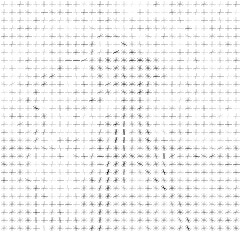
\includegraphics[width=0.5in,height=0.5in]{second_table_sobel_n5/cnoise_3.jpg}
& 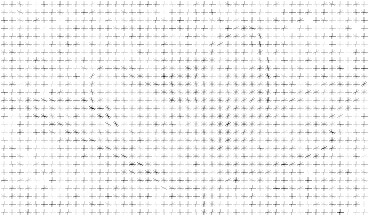
\includegraphics[width=0.5in,height=0.5in]{second_table_sobel_n5/fnoise_3.jpg}
& 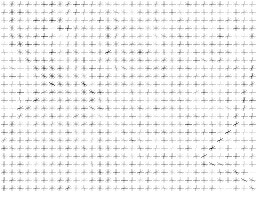
\includegraphics[width=0.5in,height=0.5in]{second_table_sobel_n5/gnoise_3.jpg}
& 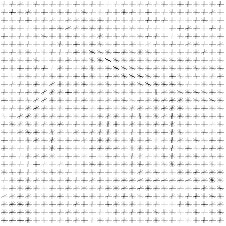
\includegraphics[width=0.5in,height=0.5in]{second_table_sobel_n5/hnoise_3.jpg}
\\ \hline \hline
\end{tabular}
\end{adjustbox}
\end{table}
%------------------------------------------------


The performances for the proposed methods I, II, and III (with $h=1$ and $n=32$) and another compared method, i.e., Sobel over four images were evaluated in table \ref{tab1}.
These results are almost identical for noise-free images.
It can be said that in the noiseless scenario, the performances of the three proposed methods I, II, and III are almost the same.
In addition, the performances of the three proposed methods I, II, and III are almost similar to that of the competing method.

In the next step, the performances of the three proposed methods I, II, III and the Sabel method for removing Gaussian noise with a power of 50 were evaluated.
According to table \ref{tab2}, the first row shows the input noisy images.
The other pictures in this table the output of four methods, respectively.
As you can see, the worst results for the Sabel method have located in the last row of this table.

%------------------------------------------------
\begin{figure*}[!th]
	\centering
	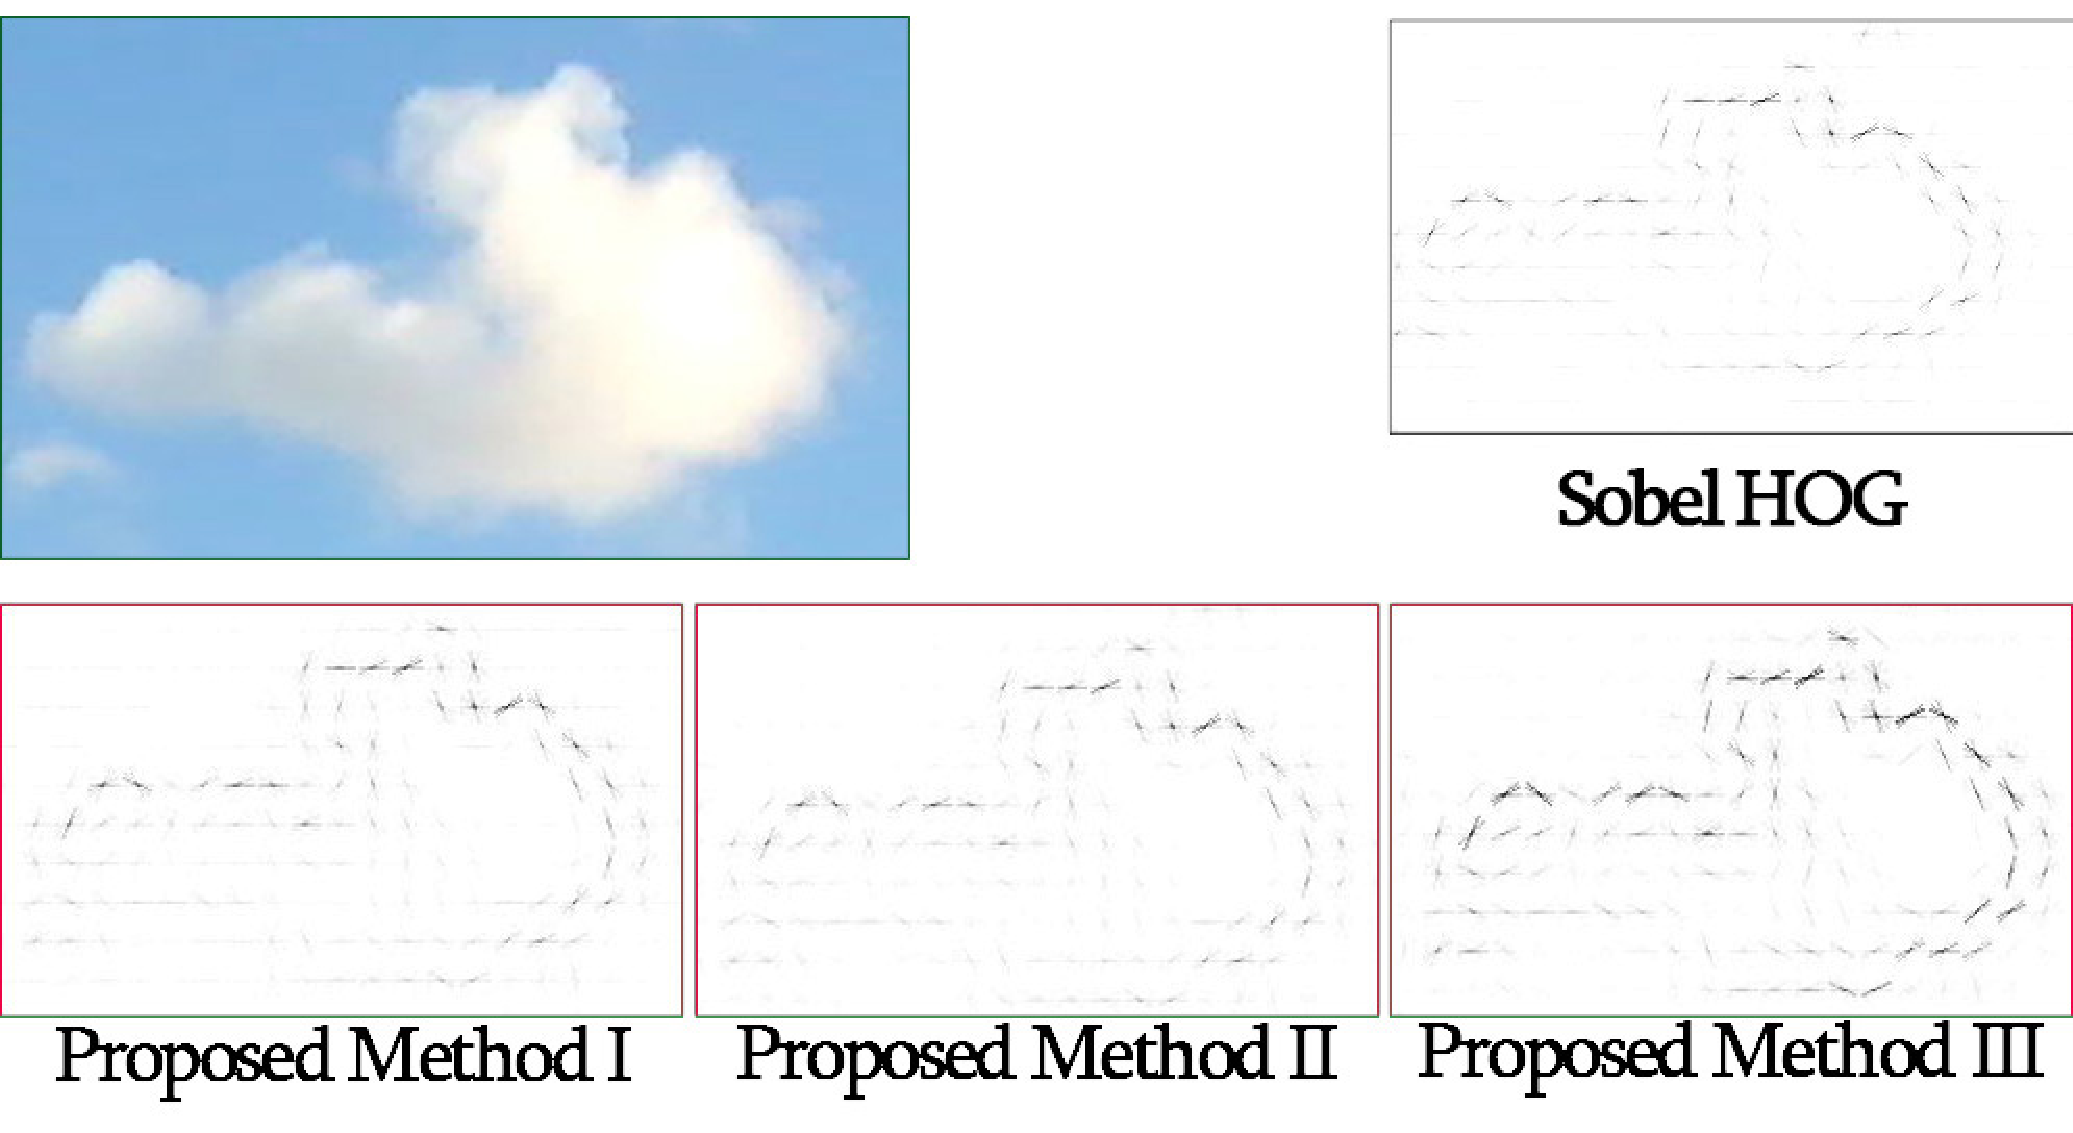
\includegraphics[height=4cm,width=8cm]{comparing_the_intensity_of_recognized_edges.pdf}
	\caption{Comparing the intensity of recognized edges for Cloud image using proposed method I, II, III and Sobel HOG method..}
	\label{New1}
\end{figure*}
%------------------------------------------------

%-------------------------------------------
\begin{figure*}[!th]
	\centering
	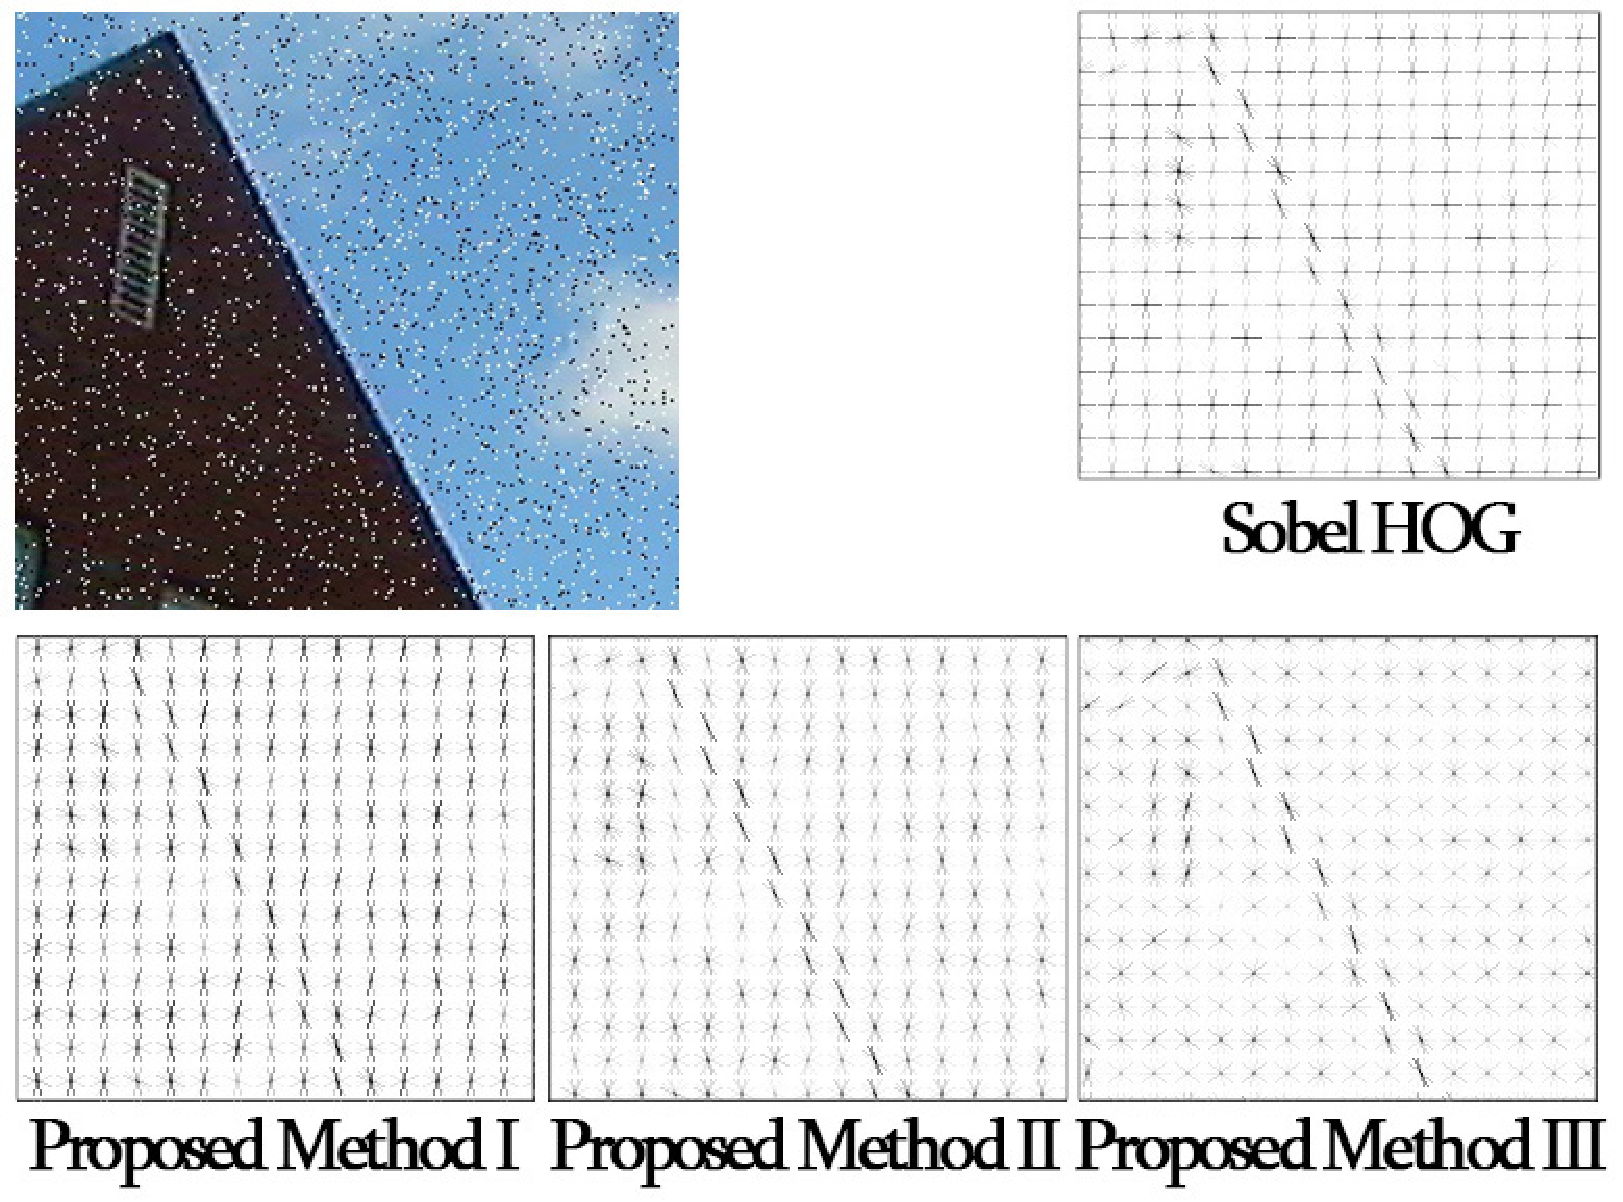
\includegraphics[height=4cm,width=8cm]{comparing_Robustness_of_images.pdf}
	\caption{Comparing the intensity of recognized edges after applying a noise of 3\% salt and pepper.}
	\label{New3}
\end{figure*}
%-------------------------------------------
%-------------------------------------------
\begin{figure*}[!th]
	\centering
	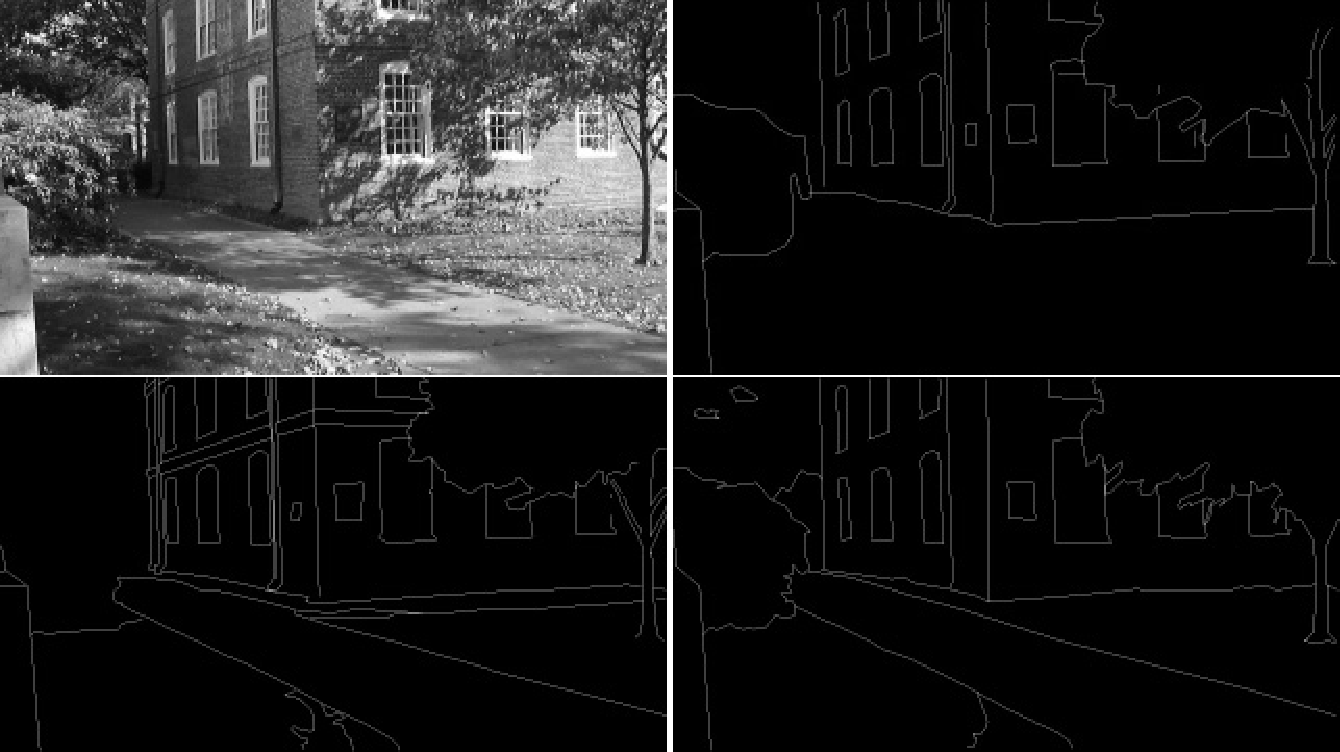
\includegraphics[height=5cm,width=12.74cm]{A_sample.pdf}
	\caption{A sample in the dataset, original picture and different edge schemes drawn.}
	\label{fig7_1224}
\end{figure*}
%-------------------------------------------
%-------------------------------------------
\begin{figure*}[!th]
	\centering
	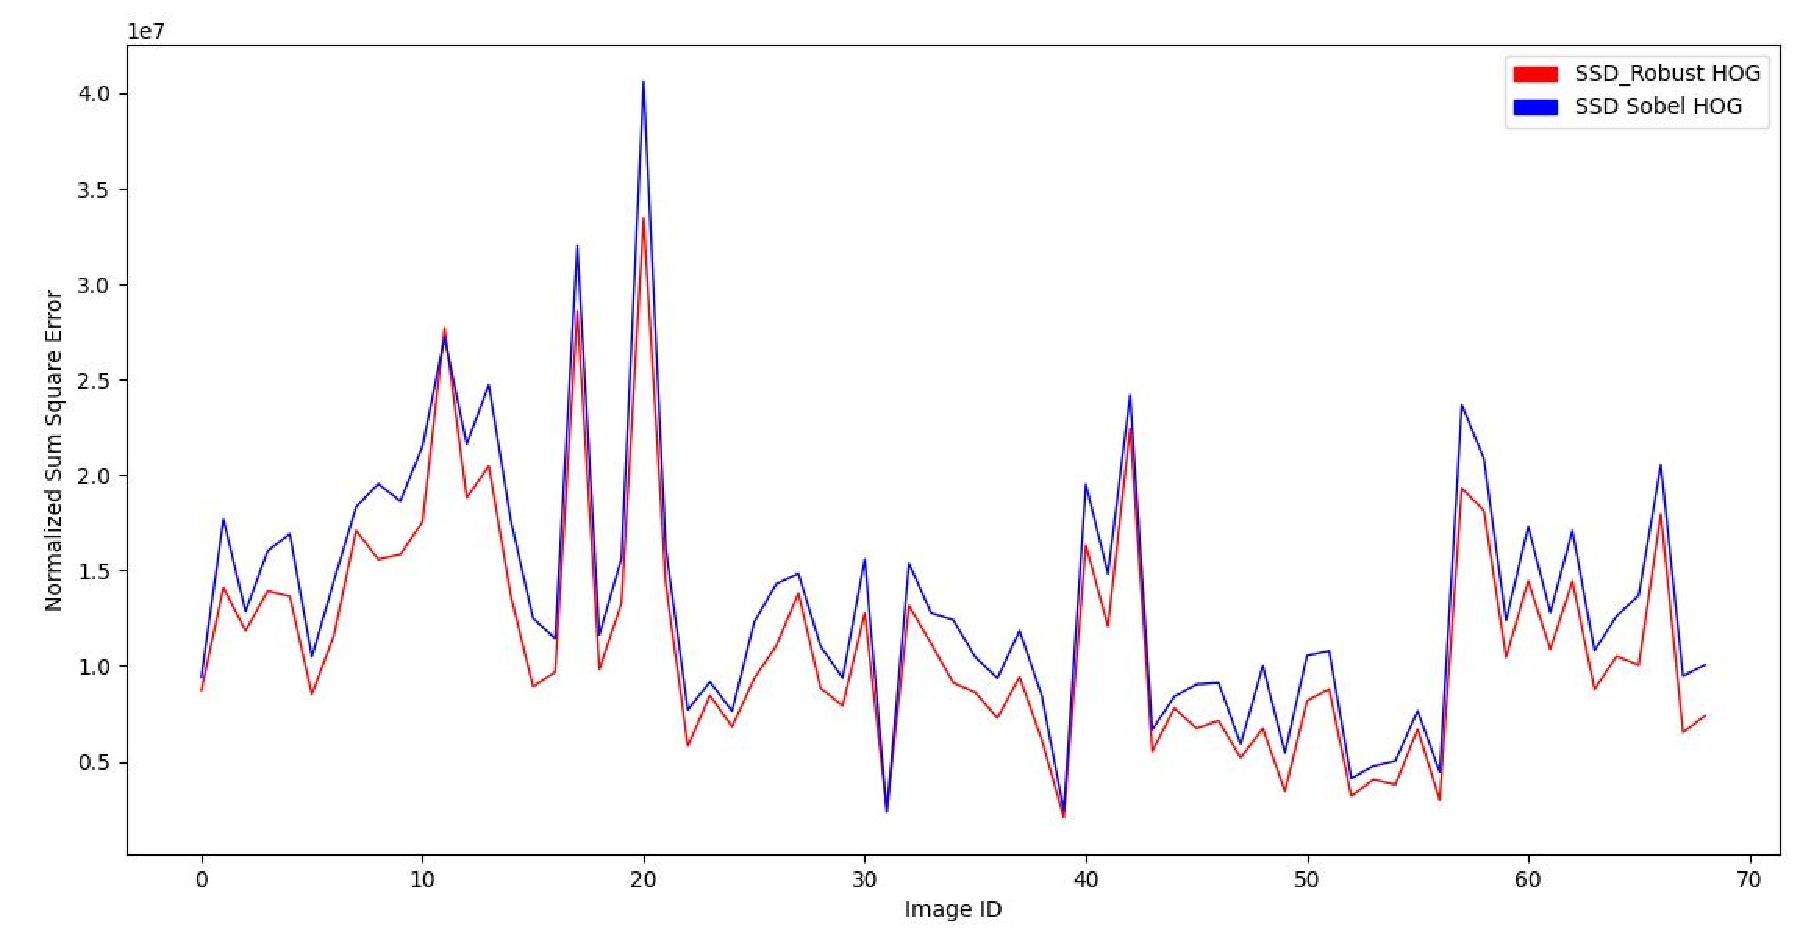
\includegraphics[height=5cm,width=12.74cm]{Sobelrobust_ssderror_gamma0_0021_h1_n8_salt5.pdf}
	\caption{Sobel and Robust SSD error with $\gamma=0.0021$, $h=1$, $n=8$ and salt pepper noise power 5\%.}
	\label{fig7_12244}
\end{figure*}
%-------------------------------------------
%-------------------------------------------
\begin{figure*}[!th]
	\centering
	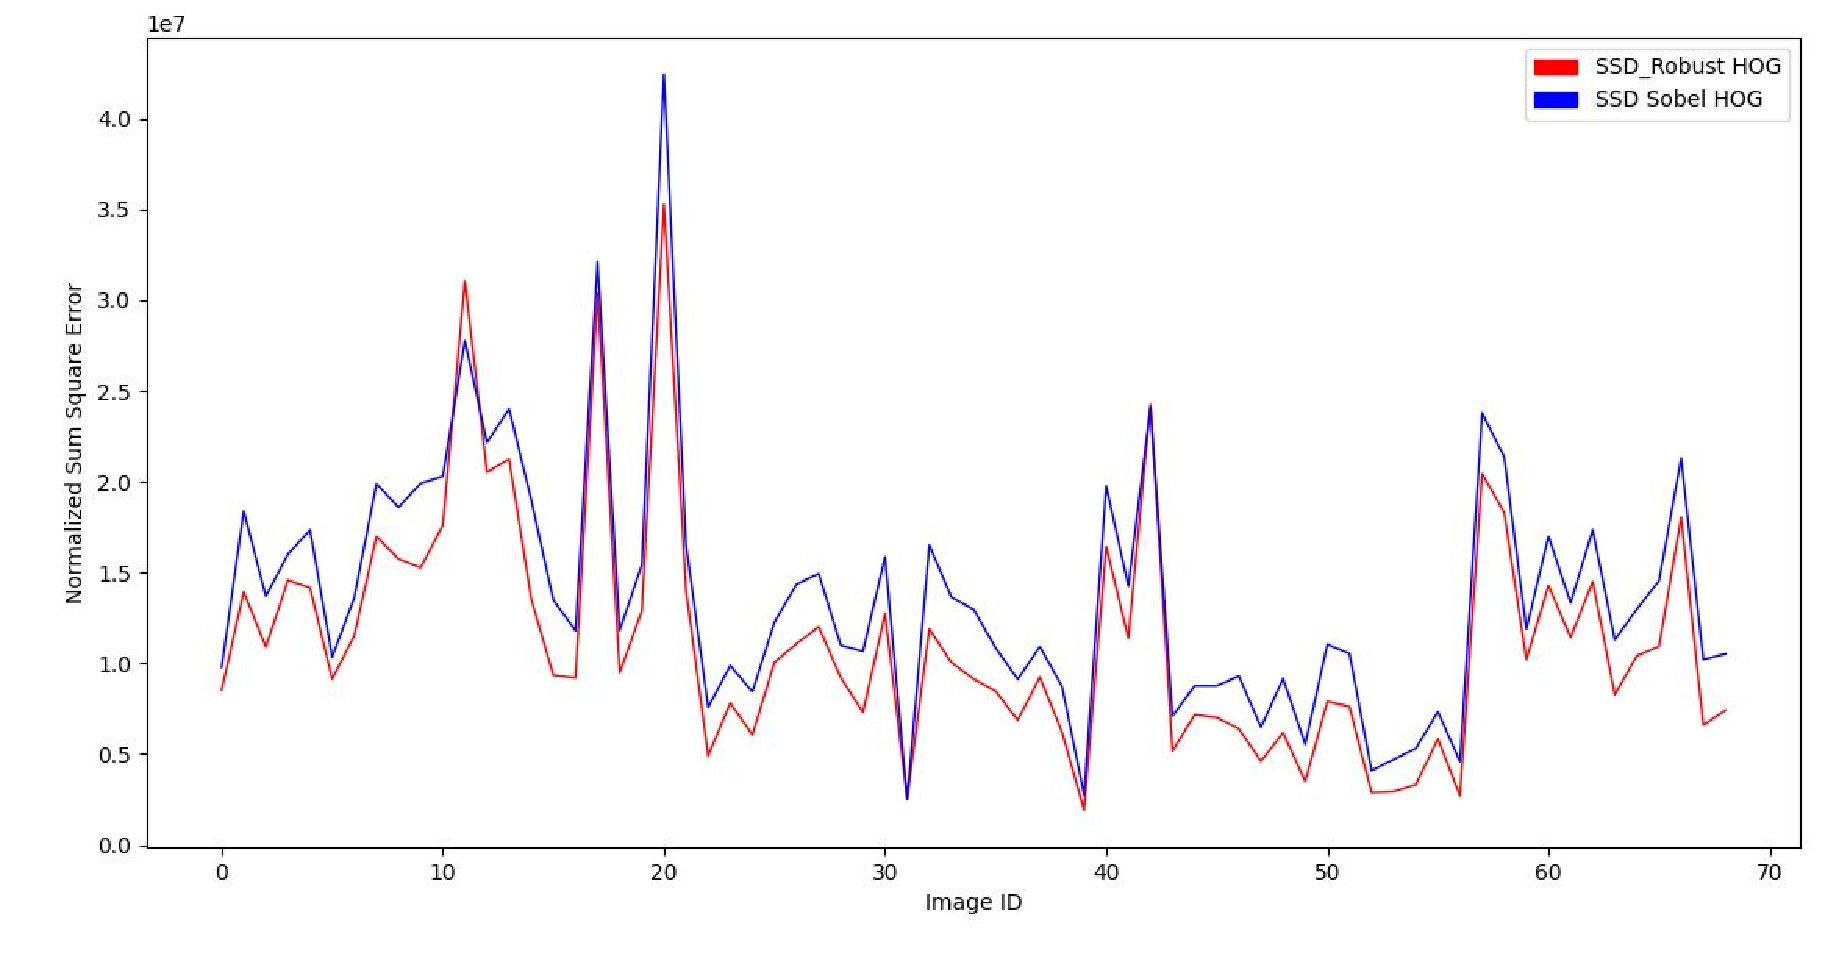
\includegraphics[height=5cm,width=12.74cm]{Sobelrobust_ssderror_gamma0_0005_h1_n16_salt5.pdf}
	\caption{$n=16$, $h=1$, $\gamma=0.0021$, tested on images with 5\% power of salt pepper noises.}
	\label{fig7_122442}
\end{figure*}
%-------------------------------------------
%------------------------------------------------
\begin{figure*}[!th]
	\centering
	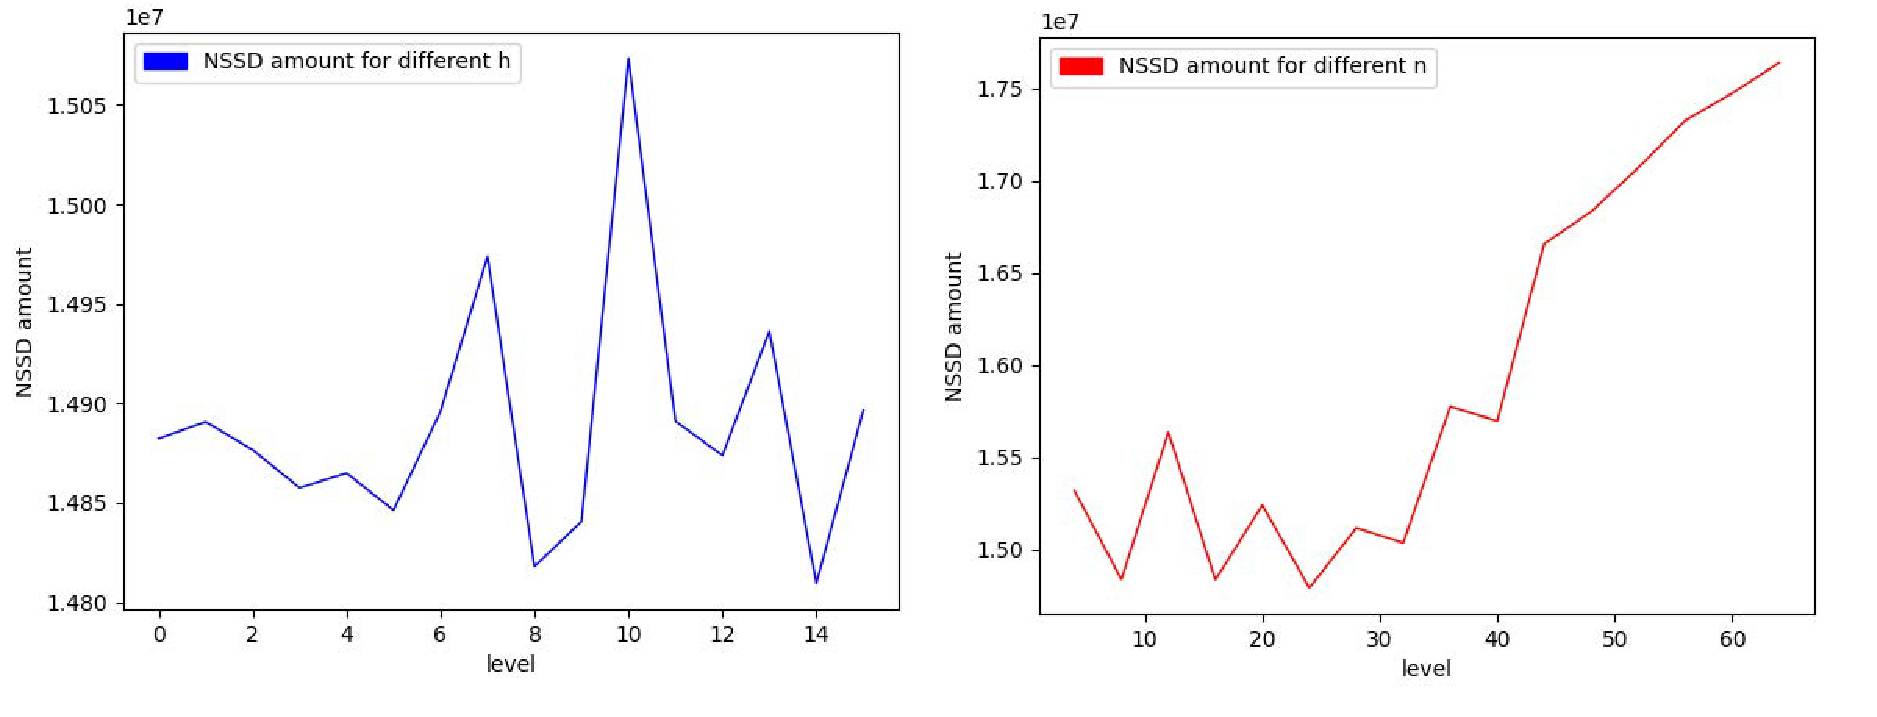
\includegraphics[height=5cm,width=12.74cm]{impact_of_different_h_and_n_on_the_NSSD_error2.pdf}
	\caption{Impact of different $h$ and $n$ on the NSSD error.}
	\label{fig7_1222}
\end{figure*}
%------------------------------------------------
Also, in table \ref{tab3} we obtained the outputs of methods for noisy images destroyed with 5\% salt and pepper noise. As can be seen, the performance of the proposed method III is much better than the other methods in the presence of noise.

For more discussion on the difference of our methods and the effect of the parameters on output, we designed an experiment on a certain image to focus on its edges.
As shown in fig. \ref{New1}, using the first algorithm, the cloud’s histogram is partially detected, while in the histogram obtained from the Sobel method, the intense of the desired cloud edges is fader than the presented histograms.
By performing optimization, focusing on the first two derivatives of the sequence, the value of the first two expressions or the first derivative in the $x$ and $y$ directions is amplified relative to the derivatives in the rest of the image, and after normalization the cloud boundaries are shown more prominently. For this reason, in the second algorithm, we can see the real boundaries more solidly than the rest of the boundaries. In the third algorithm, in addition to the previous boundaries, even new boundaries are identified with greater sensitivity. Color changing in the cloud of the main picture can be even identified as an edge in the histogram obtained by the third algorithm, which by raising n or h we will observe it more clearly in the output. 

Although the performance of the first algorithm in noise-free images is better than Sabel, its performance in noisy images is not optimal. As can be seen in the image in fig \ref{New3}, after applying a noise of 3\% salt and pepper to the image, the final output of the image in the first method is strongly affected and no border is observed in the image. The noise presented to the image makes derivatives err at several points, so the image gradient is not calculated correctly, although the effect of noise decreases as the number of terms grows, so the calculated derivative will depend on more neighboring points. In the second algorithm, the effect of noise is reduced by tuning weights, but the application of Correntropy in the third algorithm neutralizes the outlier noises. As a result, no noise is observed in the final image in the third algorithm.

In fig \ref{fig7_1224}, some conditions were equally met for both experiments. Pictures were selected from dataset (https://serre-lab.clps.brown.edu/resource/multicue/) and some of them are shown below. We consider second group of pictures, which are presenting edges using different ways to draw manually, as a base to compare our propose method and other method.
In experiments represented in figs. \ref{fig7_12244} and \ref{fig7_122442}, we tried to examine the impact of different $h$ and $n$ on the quality of pictures. In the second tests, we compare our proposed method (method III) with Sobel to find out how much our result performed better. The size of all picture were set to $320\times 160$.
After applying noises on images, we did experiments for two types of noises, salt and pepper and Gaussian noise. These experiments were done on salt and pepper noise with power of 5\%. We calculated Normalized Sum Square Difference (NSSD) in fig. \ref{fig7_1222}, for the results of the proposed method and Sobel method by using the base pictures as a real edges. NSSD is calculated by $S_eq =$ $\sigma$ $(J[n,m] - I[n,m])^2)$.
Where $\sigma$ was selected 0.0021 to have an optimal outcome for our method. It is obvious that for all images below (x-axis is showing the $id$ of each image) the amount of NSSD for our method is lower than Sobel method except one picture after testing on 70 images (rate of success 98.57\%). Two charts were calculated by changing the parameters to measure the impact of each.
The charts are gained by calculating the average of more than ten pictures.
%------------------------------------------------
\section{Conclusions}
In this paper, we presented a novel approach to design a robust HOG-based method using Maclaurin series, enhancing by the loss functions. The research based HOG feature extraction framework was performed in three approaches, i.e., the proposed methods I, II, and III, to achieve satisfactory accuracy for one-dimensional and two-dimensional signals with two different types of noise in different percentages. After the gradient calculation stage, we compute the HOG, utilizing visual presentation known as the method I. The first method illustrated an acceptable outcome while the total run-time was much lower than other methods.
In the following step, in an iterative framework based on two loss functions, i.e., least square and correntropy, we constructed the new optimization problem.
By proposing least square function, we could optimize our final results in some conditions we used noisy images. There was a great achievement in minimizing the correntropy loss function, coinciding with the increment of run-time.
To solve the problem based on the correntropy loss function, we used the half quadratic approach. So, the final results were robust against the noises, such as Salt and pepper and Gaussian noises. Eventually, we also compared our outcomes, which are visually admissible, with Sobel method.
%------------------------------------------------
%------------------------------------------------
\appendix
\section{Half Quadratic (HQ) Optimization}
To describe HQ optimization approach used in \eqref{Q26_1}, first we bring the definition of the conjugate function theory $\phi^*(z)$ for a convex function $\phi(s)$ as \cite{boyd2004convex}:
\begin{equation}\label{A1}
\begin{aligned}
&\phi^*(z)=\sup_{s\in Dom(\phi)}(z^Ts-\phi(s))
\end{aligned}
\end{equation}
where $\phi(s)=-slog(-s)+s$, $s<0$ is a convex function. By replacing this in \eqref{A1}, we have:
\begin{equation}\label{A2}
\begin{aligned}
&\phi^*(z)=\sup_{s\in Dom(\phi)}(z^Ts+slog(-s)-s)
\end{aligned}
\end{equation}
Then, to get the solution of \eqref{A2}, we set the derivation of $z^Ts+slog(-s)-s$ with respect to $s$ to zero. So, we have:
\begin{equation}\label{A3}
\begin{aligned}
&s=-exp(-z)<0
\end{aligned}
\end{equation}
By using \eqref{A3} in \eqref{A2}, the conjugate function of $\phi(s)$ is equal to $\phi^*(z)=exp(-z)$.
%------------------------------------------------
%------------------------------------------------
\section*{Reference}
\bibliography{ref}
\end{document}
%------------------------------------------------